%-------------------------------------------------------------------------------
\chapter{The Finite Volumes unsteady transcritical engine \mascaret{}}
\label{Chapter3}
%-------------------------------------------------------------------------------

%-------------------------------------------------------------------------------
\section{Introduction}
%-------------------------------------------------------------------------------

The development of the transcritical engine originated from the need to have a code to carry out studies of flood waves, that also met the associated criteria of quality and performance.

The initial objective of the transcritical engine was, therefore, to allow the calculation of :
\begin{itemize}
 \item flow in valleys with bottom slopes possibly reaching 10\% over zones of limited size, and of strong variation of width (plunging gorges, rocky constrictions, etc...);
 \item very fast flows with the presence of discontinuities ;
 \item wave propagation over dry zones ;
 \item water lines in valleys several hundreds of km in length and with the presence of tributaries;
 \item water lines with supercritical reaches and the treatment of steady flow, for such applications as the flushing of reservoirs.
\end{itemize}

The various constraints listed above resulted, at a numeric level, in the adoption of a conservative scheme (the Roe scheme with biased treatment of the source terms) allowing for discontinuous solutions.

In the first part \ref{ESVTcons}, we recall the one-dimensional equations of Saint-Venant, written in a conservative form.

The second part is devoted to the numerical solution of the homogeneous problem and the source terms for a single reach. Presented in section \ref{resNumSVT} is the solution method used in the transcritical engine of \mascaret{}, with a \textit{finite volume} scheme explicit or implicit in time.

The explicit scheme can address highly unstationary problems such as flood waves. The numerical results are satisfactory but the constraint on the time step, due to the explicit scheme, is very restrictive for slightly unstationary flows and subcritical flows. This led to implicit the initial scheme linearly.

In the third part \ref{ModelCplx}, the more complex physical developments are presented such as the modelling of the compound channels, singularities (downstream dams, weirs, etc.) and confluences.

%-------------------------------------------------------------------------------
\section{Equations of Saint-Venant in a conservative form}
\label{ESVTcons}
%-------------------------------------------------------------------------------

%...............................................................................
\subsection{General form of the equations (a reminder)}
%...............................................................................

The flow in a river can generally be considered as one-dimensional, i.e. the function of only one variable of space, the curvilinear abscissa $x$ of the river channel.

The variables of the flow are therefore the discharge $Q$ and the wetted section $S$, functions of $x$ and of time $t$, and defined in each of the vertical sections of the river.

To obtain the equations of Saint-Venant starting from the equations of Navier-Stokes, it is supposed that the angle between the bottom and the horizontal is always small. Nevertheless, in practical application, we also need to compute zones with very strong slopes, but of limited extent.

In the hypothesis where the pressure within the fluid is hydrostatic and where the internal viscosity effects are negligible compared to the friction on the walls of the channel, $Q$ and $S$ are solutions of the equations of Saint-Venant and are written as \cite{GOUTAL91} \cite{AFIF86} :

\begin{equation}
 \label{SVT2}
 \left \lbrace
  \begin{array}{l}
    \frac{\partial S}{\partial t} + \frac{\partial Q}{\partial x} = q_a \\
    \\
    \frac{\partial Q}{\partial t} + \frac{\partial}{\partial x} \left ( \frac{\beta(x,S) Q^2}{S}\right ) + g S \frac{\partial Z}{\partial x} = g S J
  \end{array}
 \right.
\end{equation}
where:
\begin{itemize}
 \item $Z$ is the elevation of the free surface ($m$);
 \item $S$ is the wetted section ($m^2$);
 \item $g$ is the acceleration of gravity ($m.s^{-2}$);
 \item $J$ is the linear head loss from friction. $J$ is evaluated with the Strickler formula :
  \begin{equation}
    J = \frac{Q^2}{K^2 S^2 R_{h}^{4/3}}
  \end{equation}
  with $R_h$ the hydraulic radius and $K$ the Strickler friction coefficient.
\end{itemize}


It is reminded that the Strickler friction coefficient $K$ is equal to $1/n$ where $n$ is the Manning friction coefficient.

\begin{figure}[H]
 \begin{center}
  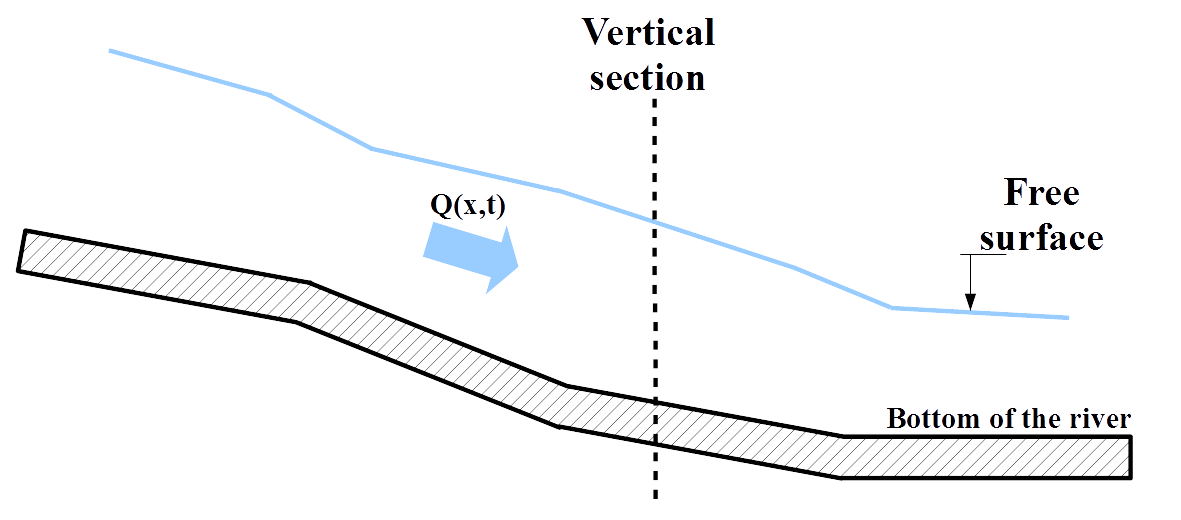
\includegraphics[width=\textwidth]{Figures/VueLong.png}
  \caption{Longitudinal view}
 \end{center}
\end{figure}

\begin{figure}[H]
 \begin{center}
  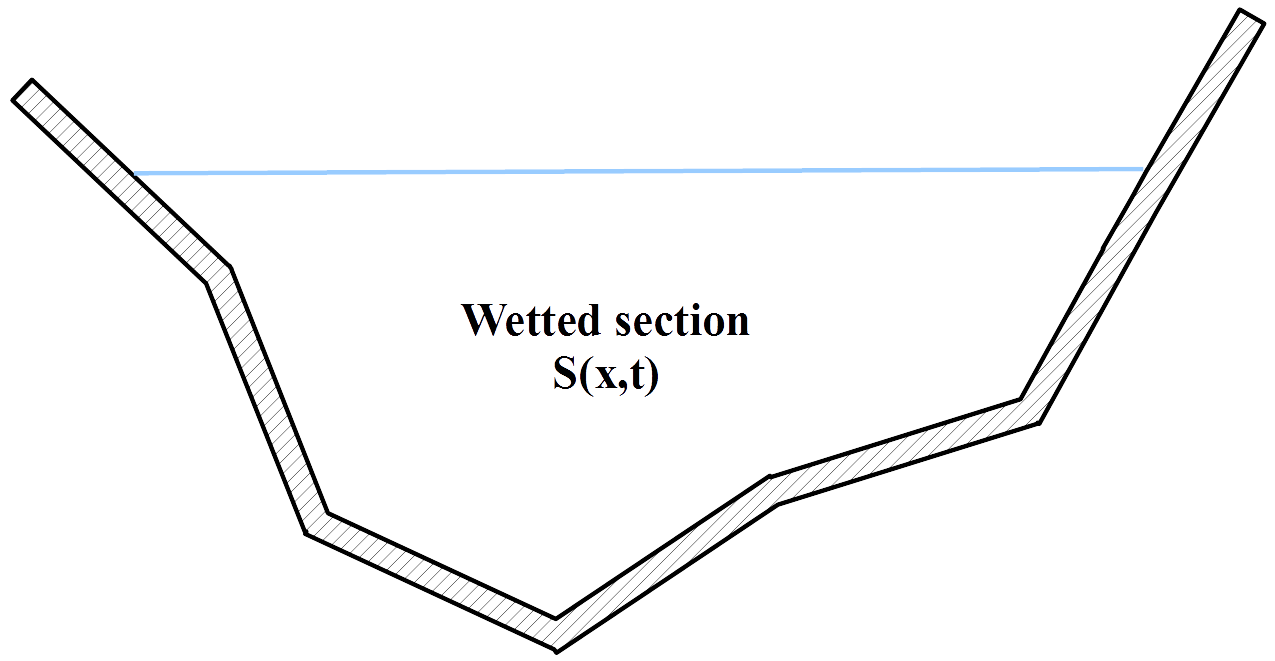
\includegraphics[width=\textwidth]{Figures/VueLat.png}
  \caption{Lateral view}
 \end{center}
\end{figure}

The dimensionless coefficient $\beta$, results from the variations of the actual velocity of the flow in a section :

\begin{equation}
 \beta(x,S) = \frac{S}{Q^2} \int V^2 \,dS
\end{equation}

In the case of a simple river channel, taking into account the hypothesis used to establish the equations of Saint-Venant, we take $\beta$ equal to 1, i.e. the variations of velocity within a section are neglected. This will not be true for a compound channel.


The system of equations (\ref{SVT2}) is obtained by expressing the conservation of mass for the first equation and the conservation of momentum for the second.

%...............................................................................
\subsection{Equations written in a conservative form}
%...............................................................................

A conservative system of equations can be expressed as :

\begin{equation}
  \frac{\partial W}{\partial t} + divF(W) = B(W)
\end{equation}
where:
\begin{itemize}
 \item $W$ is the vector of state;
 \item $F(W)$ is the flux;
 \item $B(W)$ is the source term.
\end{itemize}

Or, if there is only one dimension of space :

\begin{equation}
 \frac{\partial W}{\partial t} + \frac{\partial F}{\partial x} = B
\end{equation}

This way of writing the equation is interesting because it contains, in terms of distributions, the jump relationships in the case of a shock.

To write the conservative form of these equations from (\ref{SVT2}), we must transform the term : $g S \frac{\partial Z}{\partial x}$ in the dynamic equation. The first two terms of the dynamic equation : $\frac{\partial Q}{\partial t}$ and $\frac{\partial}{\partial x}\left ( \frac{Q^2}{S}\right )$ , correspond to the variation in momentum. This variation is equal to the action of external forces, i.e. the friction on the bottom represented by : $-g S J$ and the forces of gravity and pressure, which are taken into account by : $g S \frac{\partial Z}{\partial x}$.

The term $g S \frac{\partial Z}{\partial x}$ can be transformed by using the term for pressure : $P = g \int_{0}^{y} S \, dy$, where : $y = Z - Z_f$, $Z$ being the free surface elevation and $Z_f$ the bottom elevation.

\begin{figure}[H]
 \begin{center}
  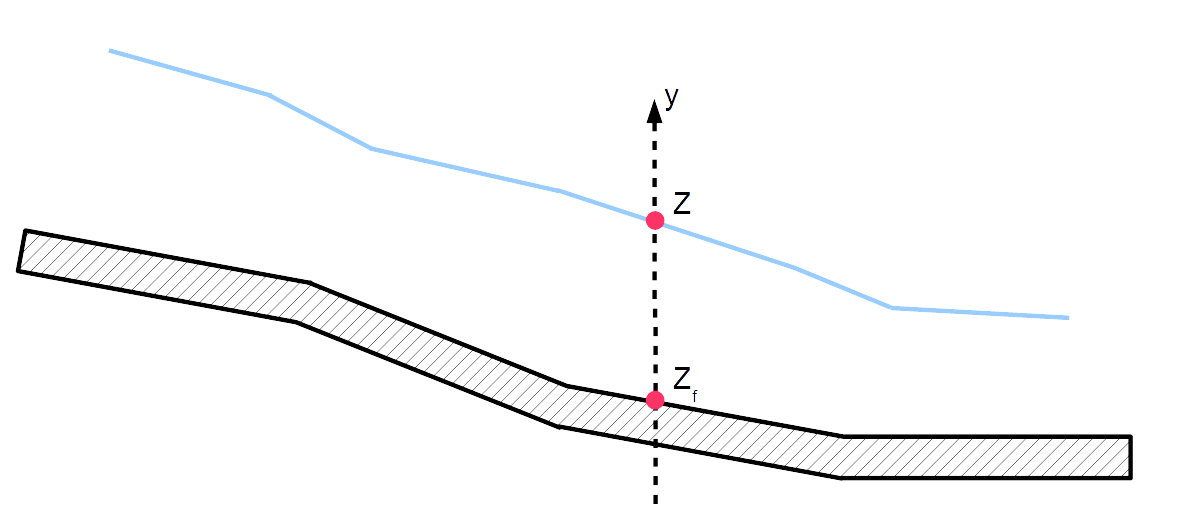
\includegraphics[width=\textwidth]{Figures/VueLong2.png}
  \caption{Longitudinal view : the elevations}
 \end{center}
\end{figure}

We can write :

\begin{equation}
 \frac{\partial P}{\partial x} = g S \frac{\partial y}{\partial x} + g \int_{0}^y \left ( \frac{\partial S}{\partial x}\right ) \, dy
\end{equation}

which is equivalent to :

\begin{equation}
 \frac{\partial P}{\partial x} = g S \frac{\partial Z}{\partial x} + g \int_{0}^y \left ( \frac{\partial S}{\partial x}\right ) \, dy - g S \frac{\partial Z_f}{\partial x}
\end{equation}

The dynamic equation can be re-written as :

\begin{equation}
 \frac{\partial Q}{\partial t} + \frac{\partial}{\partial x} \left ( \frac{Q^2}{S} + P \right ) = g \int_{0}^y \left ( \frac{\partial S}{\partial x} \right )_y \, dy - g S \frac{dZ_f}{dx} - g S J
\end{equation}

It is noted that the source term related to the geometry of the dynamic equation can equally be written : $\left( \frac{\partial P}{\partial x} \right )_{z = constant}$.

The source term of this new equation depends only on the variables $Q$ and $S$ of the geometry of the river, it does not depend on the derivative in respect to $x$ or $t$ of $Q$ and $S$. In effect, the derivative : $\left ( \frac{\partial S}{\partial x} \right )_y$ is purely geometrical (here $S$ indicates the geometric section and not the wetted section). This equation is written in a conservative form.

So, the conservative formulation of the equations of the system (\ref{SVT2}) is (with : $q_a = 0$) :

\begin{equation}
 \label{SVT3}
 \left \lbrace
  \begin{array}{l}
    \frac{\partial S}{\partial t} + \frac{\partial Q}{\partial x} = 0 \\
    \\
    \frac{\partial Q}{\partial t} + \frac{\partial}{\partial x} \left ( \frac{Q^2}{S} + P \right ) = g \int_{0}^y \left ( \frac{\partial S}{\partial x} \right )_y \, dy - g S \frac{dZ_f}{dx} - g S J
  \end{array}
 \right.
\end{equation}

with : $P = g \int_{0}^{y} S \, dy$

This equation is actually of the form :

\begin{equation}
 \frac{\partial W}{\partial t} + \frac{\partial F}{\partial x} = B
\end{equation}

with :

\begin{equation}
 W = \left ( \frac{S}{Q} \right )
\end{equation}

\begin{equation}
 F = \left (
    \begin{array}{c}
    Q \\
    \\
    \frac{Q^2}{S} + P
\end{array}
\right )
\end{equation}
and :
\begin{equation}
 B = \left (
    \begin{array}{c}
    0 \\
    \\
    g \int_{0}^y \left ( \frac{S}{x} \right )_y \, dy - g S \frac{dZ_f}{dx} - g S J
\end{array}
\right )
\end{equation}

\begin{CommentBlock}{Comment :}
\begin{itemize}
 \item The flux depends not only on $W$ but also on $x$. Knowing only $W$ is not sufficient to calculate $F$. In effect, the term for pressure $P$ appearing in $F$ can only be evaluated if the wetted section and the variation of the section based on the flow depth are known explicitely. However the variation of the section depends on the geometry of the river. Therefore it can only be know if the $x$ axis is given. We will see the importance of this statement in the search for the Riemann invariants of the system of equations (\ref{SVT3});
 \item The variables $Q$ and $S$ can be discontinuous (e.g. in the case of a hydraulic jump). The derivatives appearing in (\ref{SVT3}) therefore need to be understood in the sense of distributions. Actually, in this case, the system (\ref{SVT3}) is the only correct equation system, because in (\ref{SVT2}) the term : $g S \frac{\partial Z}{\partial x}$ has no meaning, both in a classical sense and in the sense of the distributions.
\end{itemize}
\end{CommentBlock}

%...............................................................................
\subsection{Riemann invariants}
%...............................................................................

The system (\ref{SVT3}) is hyperbolic. The jacobian matrix of $F$ : $\left ( \frac{\partial F}{\partial W} \right )_x$  admits two real and distinct eigenvalues : $\lambda^+$ et $\lambda^-$ :

\begin{equation}
 \left ( \frac{\partial F}{\partial W} \right )_x = \left (
    \begin{array}{c c}
    0 & 1\\
    \\
    -\frac{Q^2}{S^2} + \left ( \frac{\partial P}{\partial S} \right )_x & \frac{2 Q}{S}
\end{array}
\right )
\end{equation}

\begin{equation}
 \left \lbrace
  \begin{array}{l}
    \lambda^+ = \frac{Q}{S} + C \\
    \\
    \lambda^- = \frac{Q}{S} - C \\
  \end{array}
 \right.
\end{equation}

with :

\begin{equation}
 C = \sqrt{\left ( \frac{\partial P}{\partial S} \right )_x}
\end{equation}

The celerity $C$ is only a function of $S$ and $x$.

In using the properties of the hyperbolic systems \cite{GODLEWSKI91}\cite{AFIF86}, (\ref{SVT3}) can be rewritten in the form of two convection equations of the Reiman invariants.

We do not give the details of the calculations here (see \cite{GODLEWSKI91} and \cite{AFIF86}).

We finally obtain the system (\ref{SVT4}) :

\begin{equation}
 \label{SVT4}
 \left \lbrace
  \begin{array}{l}
    \frac{df^-}{dt} = - \lambda^- \int_{0}^S \frac{1}{S} \left ( \frac{\partial C}{\partial x}\right )_S dS - g \left ( \left ( \frac{\partial y}{\partial x} \right )_S + \frac{dZ_f}{dx} + J \right ) \\
    \\
    \frac{df^+}{dt} = + \lambda^+ \int_{0}^S \frac{1}{S} \left ( \frac{\partial C}{\partial x}\right )_S dS - g \left ( \left ( \frac{\partial y}{\partial x} \right )_S + \frac{dZ_f}{dx} + J \right )
  \end{array}
 \right.
\end{equation}

where :
\begin{itemize}
 \item $\frac{df^-}{dt} = \frac{\partial f^-}{\partial t} + \lambda^- \frac{\partial f^-}{\partial x}$ is the derivative of the Reimann invariant : $f^- = \frac{Q}{S} - K$ with $K = \int_{0}^S \frac{C}{S} \, dS$ along the characteristic curve $C^-$ of slope : $\frac{dx}{dt} = \lambda^-$;
 \item $\frac{df^+}{dt} = \frac{\partial f^+}{\partial t} + \lambda^+ \frac{\partial f^+}{\partial x}$ is the derivative of the Reimann invariant : $f^+ = \frac{Q}{S} + K$ along the characteristic curve $C^+$ of slope : $\frac{dx}{dt} = \lambda^+$.
\end{itemize}

We refer to the subcritical characteristic as the curve $C^+$, and to the supercritical characteristic as the curve $C^-$.

Expressing (\ref{SVT3}) in the form of equations along the characteristic curves is equivalent to considering two mobile markers moving along the characteristics. The discharge and the wetted section at a point in the channel at a given time, are determined by the information provided by the characteristics $C^+$ and $C^-$ which intersect at this point.

\begin{figure}[H]
 \begin{center}
  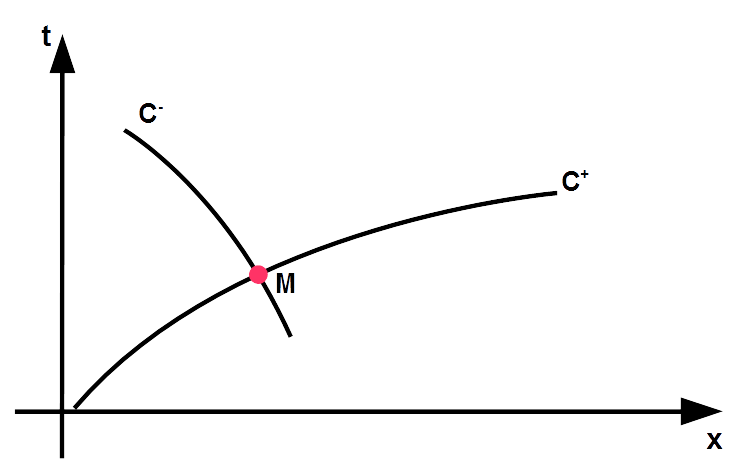
\includegraphics[width=0.8\textwidth]{Figures/2Carac.png}
  \caption{The two characteristic curves}
 \end{center}
\end{figure}

Knowing $f^+$ and $f^-$ (calculated with the help of the information conveyed by the characteristics in $M$), we can deduce $Q$ and $S$.

Formulating the system (\ref{SVT3}) in the form of characteristics also allows it to remain \textit{related} to the physical problem during the computational process. We will see an interesting application of this during the processing of the boundary conditions (see section \ref{PriseCL}).

However, the system (\ref{SVT4}) is only equivalent to the system (\ref{SVT3}) when the flow has no discontinuities. The development of the derivative $\frac{\partial F}{\partial x}$ used to obtain the system (\ref{SVT4}) is not possible in the presence of a discontinuity.

%...............................................................................
\subsection{The hydraulic jump}
%...............................................................................

\begin{CommentBlock}{Note :}
we use the terms \textit{hydraulic jump} and \textit{shock} indifferently when describing a discontinuity.
\end{CommentBlock}

A shock appears in a flow when two characteristics of the same family intersect. Two types of shock exist :
\begin{itemize}
 \item the one due to the intersection of characteristics $C^-$ : shock $C^-$;
 \item the other due to the meeting of characteristics $C^+$ : shock $C^+$.
\end{itemize}

At the point where the characteristics meet, two values of $f^-$ (for a $C^-$ shock) or two values of $f^+$ (for a $C^+$ shock) are introduced, in addition to the information derived from the other family of characteristics. This overload of information, mathematically unacceptable, results in a discontinuity at the intersection. From a physical point of view it results in the establishment of a dissipative process : the hydraulic jump.

\begin{figure}[H]
 \begin{center}
  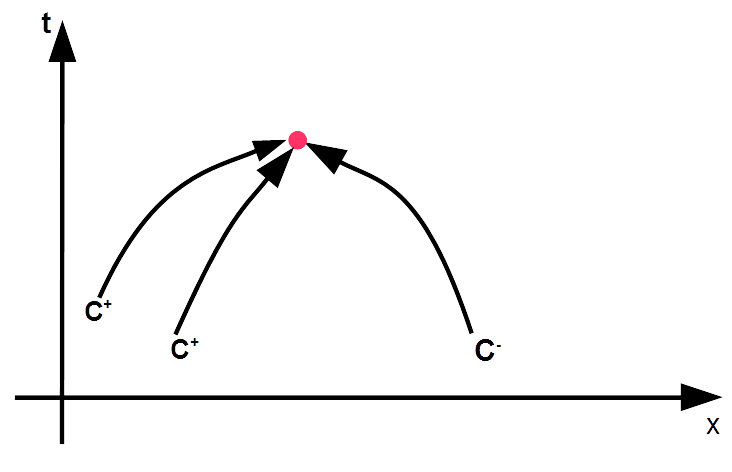
\includegraphics[width=\textwidth]{Figures/3Carac.png}
  \caption{Example of a $C^+$ shock}
 \end{center}
\end{figure}

The trajectory of the shock is made of all the points where characteristics of the same family intersect.

\begin{figure}[H]
 \begin{center}
  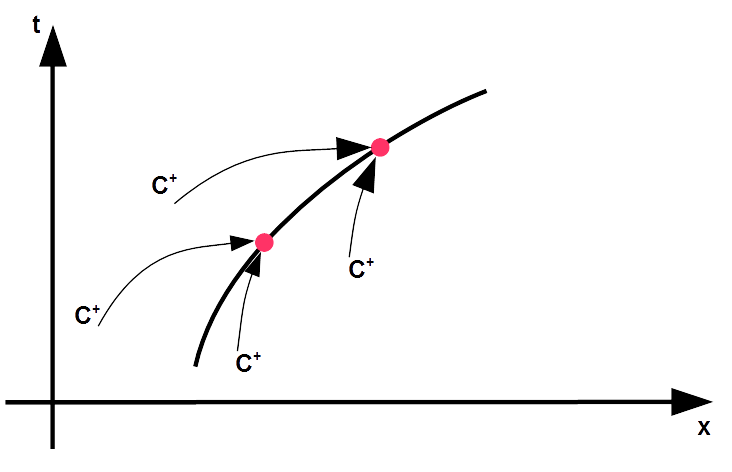
\includegraphics[width=\textwidth]{Figures/Trajec_Choc.png}
  \caption{Trajectory of a $C^+$ shock}
 \end{center}
\end{figure}

To the left and to the right of the shock, the matrix $\left ( \frac{\partial F}{\partial W} \right )_x$ is well defined, it is similarly true for its eigenvalues which are $(\lambda_{g}^+,\lambda_{g}^-)$ to the left and $(\lambda_{d}^+,\lambda_{d}^-)$ to the right.

The speed $s^-$ of a $C^-$ shock verifies :
\begin{equation}
  \left \lbrace
  \begin{array}{l}
    \lambda_{d}^- < s^- < \lambda_{g}^- (< \lambda_{g}^+) \\
    s^- < \lambda_{d}^+
  \end{array}
 \right.
\end{equation}

and the speed $s^+$ of a $C^+$ shock verifies :
\begin{equation}
  \left \lbrace
  \begin{array}{l}
    (\lambda_{d}^- < ) \lambda_{d}^+ < s^+ < \lambda_{g}^+  \\
    \lambda_{g}^- < s^+
  \end{array}
 \right.
\end{equation}

Indeed, the characteristics that create the shock catch this shock up from upstream (here to the left) and are caught up by it on the downstream (here on the right). This is the meaning of the first inequalities for the $C^-$ shocks and the $C^+$ shocks : the speed of the shock is intermediate between those of the characteristics that create it. The meaning of the second inequalities is that there cannot be a $C^-$ and a $C^+$ at the same point : the velocity of a shock cannot be between the velocities of characteristics that did not take part in its creation.

Therefore, the scheme shown in figure \ref{fig:Timp} will never be found.

\begin{figure}[H]
 \begin{center}
  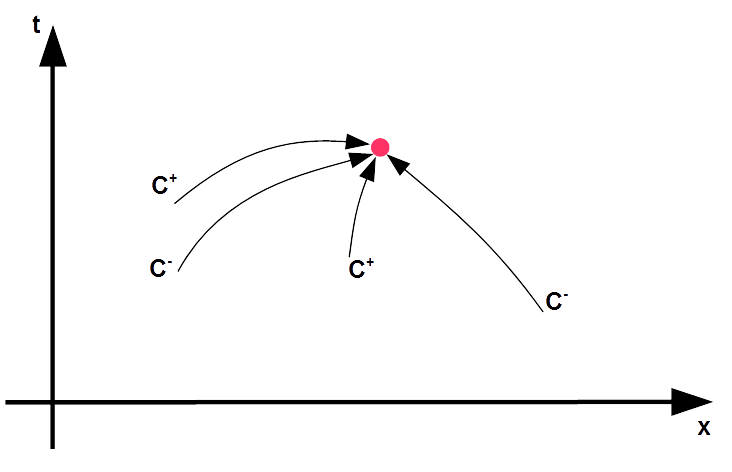
\includegraphics[width=\textwidth]{Figures/Trajec_imposs.png}
  \caption{Example of a characteristics scheme that is not possible}
  \label{fig:Timp}
 \end{center}
\end{figure}

These inequalities are all the information that the characteristics provide about the shock. Originating from a non-conservative formulation of the equations, they do not lead to a quantitative description of shocks. The states to the left and the right of a shock can not be determined by the Riemann invariants provided by the characteristics intersecting at the shock. However, for weak shocks, the speed of a shock is the average of the speed $\lambda_g$ and $\lambda_d$ of the characteristics that create it \cite{SMOLLER83}\cite{LAX72}).

The only way to describe shocks correctly is to come back to the equations written in a conservative form. When the flow contains a hydraulic jump, the homogeneous hyperbolic system, interpreted in the sense of distributions, allows to connect the states to the left and right of the hydraulic jump \cite{GODLEWSKI91}.

The relations thereby obtained are the jump conditions (these are also sometimes called Rankine-Hugoniot conditions). They are written as, with $s$ is the celerity of the hydraulic jump :

\begin{equation}
   \left \lbrace
  \begin{array}{l}
   s ( S_d -S_g ) = Q_d - Q_g \\
   s ( Q_d - Q_g ) = \left ( \frac{Q_{d}^2}{S_d} + P_d \right ) - \left ( \frac{Q_{g}^2}{S_g} + P_g \right )
  \end{array}
 \right.
\end{equation}

\begin{figure}[H]
 \begin{center}
  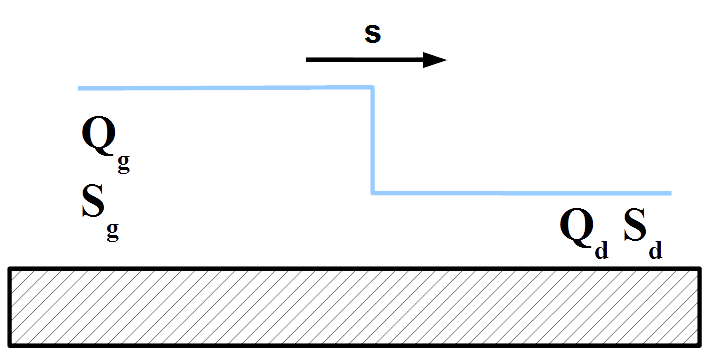
\includegraphics[width=\textwidth]{Figures/vitesse.png}
  \caption{Celerity of the hydraulic jump}
 \end{center}
\end{figure}

\begin{CommentBlock}{Comments :}
\begin{itemize}
 \item The Rankine-Hugoniot conditions are only a particular form of the system of equations (\ref{SVT3}). This can be demonstrated by doing a balance of the mass and the momentum over a slice of fluid including the hydraulic jump. In the equation of momentum, the source term disappears when the width of the slice tends towards zero.
 \item In the coordinate system of the hydraulic jump (in translation at speed $s$), the discontinuity always separates a supercritical flow from a subcritical flow. \\ In the frame of reference of the hydraulic jump : $s = 0$, so : $Qd = Qg = Qrel$ relative discharge.\\
The function :$f(S,x) = \frac{Q_{rel}^2}{S} + P$ has the same value on both sides of the jump.\\
Moreover $f$ admits a minimum for $S$ such that : $\left ( \frac{\partial f}{\partial S}\right )_x = 0$, i.e. : $Q_{rel} = C S$. The value of : $S = \frac{Q_{rel}}{C}$ corresponds to a critical flow (Froude number equal to 1). Two values of $S$ giving the same value of f (Rankine-Hugoniot condition) are therefore located on each side of the critical section.
\end{itemize}
\end{CommentBlock}

%-------------------------------------------------------------------------------
\section{Numerical solution of the St-Venant equations}
\label{resNumSVT}
%-------------------------------------------------------------------------------

%...............................................................................
\subsection{The explicit scheme}
\label{SchemExp}
%...............................................................................

In this section, we describe the numerical methods used in \mascaret{} to solve the system of equations (\ref{SVT3}). A explicit scheme was developed first, then the transcritical engine was made implicit. This leaves the choice of using one of the two schemes to the user.

%...............................................................................
\subsubsection{Description of the problem}
%...............................................................................

The system to solve is as follows :

\begin{equation}
   \label{sys}
   \left \lbrace
  \begin{array}{l}
   W = (S,Q) \\
   \\
   \frac{\partial W}{\partial t} + \frac{\partial F(W,x)}{\partial x} = B(x,W) \qquad (x,t) \in [a,b] \times [0,T]
  \end{array}
 \right.
\end{equation}

with :

\begin{equation}
 F(x,W) = \left ( \begin{array}{c}
    Q\\
    \\
    \frac{Q^2}{S} + P(x,S)
\end{array}
\right )
\end{equation}

and :

\begin{equation}
 B(x,W) = \left ( \begin{array}{c}
    0\\
    \\
    g \int_{0}^y \left ( \frac{\partial S}{\partial x} \right )_y \, dy - g S \frac{dZ_f}{dx} - g S J
\end{array}
\right )
\end{equation}

So that this problem is well presented, it is necessary to add an initial condition and boundary conditions.

The problem (\ref{sys}) to be solved, is a strictly hyperbolic system where the source term is dominant in the calculation of the flow (see the previous section).
Considering that the scope of application of the \mascaret{} code is primarily the calculation of flood waves, this implies :
\begin{itemize}
 \item geometry with very steep slopes (locally reaching $10\%$ possibly) and large variations of width;
 \item very fast flows (speeds above $10 m/s$);
 \item wave propagation over dry areas;
 \item very long computational domains.
\end{itemize}

In addition to the flood wave calculations, the intention is to be able to model any flow presenting a supercritical regime such as the flushing of reservoirs and the steady flows in torrents. This adds an additional constraint, which is that the source term must be correctly calculated in order to obtain a correct convergence towards steady flows. The objective was to find a scheme that complies with these various constraints (which can sometimes be contradictory) as closely as possible.
\vspace{0.5cm}

For now we are interested only in the numerical solution of the homogeneous problem. A following section, \ref{TrtSource} is devoted to the treatment of the source terms.

%...............................................................................
\subsubsection{Solution of the homogeneous problem}
\label{PbHom}
%...............................................................................

The homogeneous problem to solve is written :

\begin{equation}
 \frac{\partial W(x,t)}{\partial t} + \frac{\partial F(W)}{\partial t} = 0
\end{equation}

This homogeneous problem is very similar to the isentropic Euler equations. The principle difference resides in the fact that the flux does not depend solely on the state variables (which are the wetted section and the discharge) but also depends on the variable of space $x$. Moreover, the pressure term is not known explicitely but is a tabulated variable.

The time interval $[0,T]$ is discretised in a series of intervals $[t_n , t_{n+1}]$ with : $t_{n+1} = t_n + \Delta t$ where $\Delta t$ is the time step.

The computational domain will be discretised in $N$ intervals $[x_i , x_{i+1}]$ with : $\Delta x_i = x_{i+1} - x_i$.

We denote $x_{i+1/2}$ the midpoint of the interval $[x_i , x_{i+1}]$.

The scheme used is a finite volume scheme based on a integral formulation of the mass and momentum balance over a cell $[x_{i-1/2},x_{i+1/2}]$ (see figure \ref{fig:Schm1}).

\begin{figure}[H]
 \begin{center}
  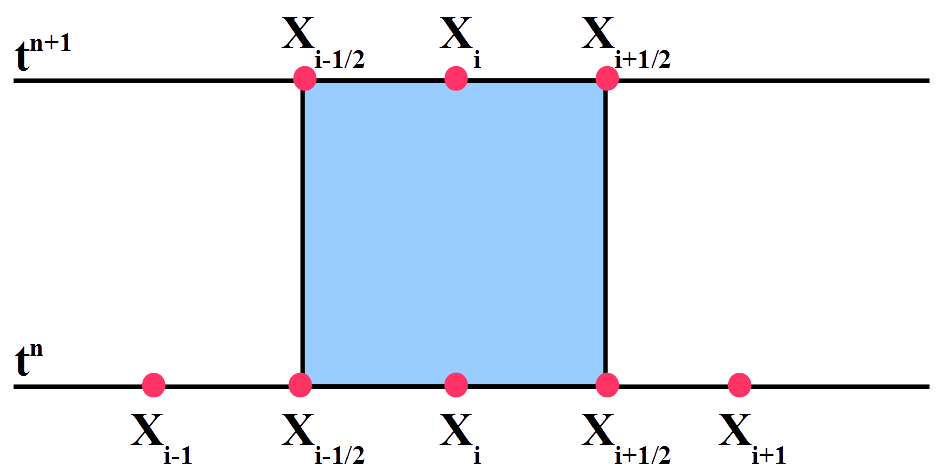
\includegraphics[width=\textwidth]{Figures/Schema1.png}
  \caption{Finite volume cell}
  \label{fig:Schm1}
 \end{center}
\end{figure}

\begin{CommentBlock}{Note :}
$\underline{W}_h = \left \lbrace \Psi_h \in L^2 (\Omega), \Psi_{h/]x_{i-1/2},x_{i+1/2}[} = constant, i = 1..N \right \rbrace$
\end{CommentBlock}

A variational description of the problem (\ref{sys}) can be formulated as :

find $W_h(S_h,Q_h) \in \underline{W}_h$ such as :

\begin{equation}
 \label{fvar}
 \int_{t_n}^{t_{n+1}} \int_{a}^{b} \left ( \frac{\partial W_h}{\partial t} + \frac{\partial F(x,W_h)}{\partial x} \right ) \Psi_h \, dx \, dt = 0 \qquad \forall \Psi_h \in \underline{W}_h
\end{equation}

Each function $\Psi_h$ of $\underline{W}_h$ is determined in a unique way by :

\begin{equation}
 \Psi_h = \sum_{i=1}^n \Psi (a_i)\phi_i
\end{equation}
with $\left \lbrace \varphi_i\right \rbrace_{i=1,N}$ which forms a base of $\underline{W}_h$. In fact, the functions of base $\varphi_i$ are the characteristic functions of the interval $[x_{i-1/2},x_{i+1/2}]$.

By writing the variational equation (\ref{fvar}) for each base function and by using the Green formula, we obtain :

\begin{eqnarray}
 & \int_{x_{i-1/2}}^{x_{i+1/2}} W_{h}^{n+1}\, dx = \int_{x_{i-1/2}}^{x_{i+1/2}} W_{h}^{n}\, dx + \int_{t^n}^{t^{n+1}} F(x_{i+1/2},W_{i+1/2}) \, dt  &         \nonumber \\
 & - \int_{t^n}^{t^{n+1}} F(x_{i-1/2},W_{i-1/2}) \, dt &
\end{eqnarray}

$W_{h}^{n+1}$ being sought in the space of the functions that are constant per cell, the previous equation becomes :

\begin{eqnarray}
 & W_{i}^{n+1} = W_{i}^n + \frac{1}{x_{i+1/2}-x_{i-1/2}} & \nonumber \\
 & \times \left ( \int_{t^n}^{t^{n+1}} F(x_{i+1/2},W_{i+1/2}) \, dt - \int_{t^n}^{t^{n+1}} F(x_{i-1/2},W_{i-1/2}) \, dt \right ) &
\end{eqnarray}

The problem can therefore be reduced to the evaluation of the numerical flux at each interface. Moreover, $W_{n+1}$ being a function constant per cell, the calculation of the numerical flux will require the solution of a Riemann problem at each interface.

Therefore, at each time step and each cell interface, the following problem needs to be solved :

\begin{equation}
 \label{sysW}
 \left \lbrace
  \begin{array}{l}
   \frac{\partial W_h}{\partial t} + \frac{\partial F(x_{i+1/2},W_h)}{\partial x} = 0 \\
   \\
   W_{h}^n = \left \lbrace
             \begin{array}{l}
               W_{i}^n \qquad \mbox{si} \quad x < x_{i+1/2} \\
               W_{i+1}^n \qquad \mbox{si} \quad x > x_{i+1/2}
             \end{array}
             \right.
  \end{array}
 \right.
\end{equation}

To solve this problem, it is natural to consider a Godunov scheme, based on the exact solving of the Riemann problem at each interface. However, the interest of this exact solution is counterbalanced by the fact that firstly the projection on each cell can cause a loss of quality from the exact solving, and secondly an exact Rieman solver is computationally expensive. For this reason an approximate Riemann solver has been chosen. More specifically, we have retained the Roe scheme which will be presented in the following paragraph. Moreover, another reason to choose the Roe scheme is that it is widely used for solving Euler and Saint-Venant equations \cite{PAQUIER95}\cite{VAZQUEZ94}\cite{AMBROSI95}\cite{MONTHE97}.

%...............................................................................
\subsubsection{Roe linearisation}
\label{LinRoe}
%...............................................................................

The aim here is to define a Riemann problem \textit{close} to (\ref{sysW}) but for which the solution is simpler to calculate. To do this, we apply the Roe linearisation method. This method is well known and widely used. We recall the main references where the reader can find the details of the calculation of the Roe linearisation \cite{ROE81}\cite{BUFFARD93}.

The principle of the Roe linearisation method rely on the fact that there exists a matrix A (called 'Roe linearised') verifying :
\begin{itemize}
 \item[*] $F(W_g) - F(W_d) = A(W_g,W_d)(W_g-W_d)$;
 \item[*] $A(W,W) = DF_{w}(W)$;
 \item[*] the matrix $A(W,W)$ has real eigenvalues and the eigenvectors generate the complete space.
\end{itemize}

\begin{CommentBlock}{Comment: }
The Roe linearisation method defined here is only valid for cases were the flux F depends solely on the state variables. Nevertheless, this method has been applied in the present case.
\end{CommentBlock}

The Roe scheme cannot be used if it is not possible to find a matrix satisfying these three properties. In this context, the difficulty lies with the fact that the flux depends on $x$ and the state variables.

To calculate the Roe matrix, the method is similar to that used for the isentropic Euler equations i.e. an average state is sought, so that the Roe matrix is the jacobian matrix of the flux taken in that average state.

In our case, the average of Roe $\tilde W$ is given by :
\begin{equation}
 \tilde W = \frac{W_g \sqrt{S_g} + W_d \sqrt{S_d}}{\sqrt{S_g} + \sqrt{S_d}}
\end{equation}
where :
\begin{itemize}
 \item $W_g \left ( \begin{array}{c}
    S_g\\
    V_g
    \end{array} \right )$ indicates the state to the left;
 \item and $W_d \left ( \begin{array}{c}
    S_d\\
    V_d
    \end{array} \right )$ the state to the right;
\end{itemize}

The Roe matrix $\tilde A (x,W_g,W_d)$ is the jacobian $A(x,W)$ calculated in this state.

\begin{equation}
 A(x,\tilde W) = \left ( \begin{array}{cc}
       0 & 1 \\
       \frac{-\tilde{Q}^2}{\tilde{S}^2} + \frac{\partial P(x,\tilde S )}{\partial S} & 2 \frac{\tilde Q}{\tilde S}
    \end{array} \right ) \quad \mbox{with } \tilde W (\tilde S , \tilde Q)
\end{equation}

The Riemann problem is therefore equivalent to the following linearised problem at each interface :

\begin{equation}
 \label{sysW2}
 \left \lbrace
  \begin{array}{l}
   \frac{\partial W(x,t)}{\partial t} + \tilde A(x_{i+1/2},W_g,W_d) \frac{\partial W(x,t)}{\partial x} = 0 \\
   \\
   W(x,t^n) = \left \lbrace
             \begin{array}{l}
               W_{g} \quad \mbox{si : } x < x_{i+1/2} \\
               W_{d} \quad \mbox{si : } x > x_{i+1/2}
             \end{array}
             \right.
  \end{array}
 \right.
\end{equation}

with : $\tilde A(x_{i+1/2},W_g,W_d) = A(x_{i+1/2},\tilde W)$

The solution of the linear problem (\ref{sysW2}) will allow the Roe scheme to be fully explicited.

\begin{CommentBlock}{Comment :}
The Roe matrix is evaluated at the interface $x_{i+1/2}$.
\end{CommentBlock}

%...............................................................................
\subsubsection{The Roe solver}
%...............................................................................

The solution of the problem (\ref{sysW2}) is simple. It consists of 3 constant states separated by jumps through the characteristics defined by :

\begin{equation}
  \frac{x}{t}=\lambda_{1,2}
\end{equation}

with :

\begin{equation}
 \lambda_1(x,S,Q) = \frac{Q}{S} - C(x,S)
\end{equation}

\begin{equation}
 \lambda_2(x,S,Q) = \frac{Q}{S} + C(x,S)
\end{equation}

and :

\begin{equation}
 C(x,S) = \frac{\partial P(x,S)}{\partial S}
\end{equation}

We can note that :
\begin{equation}
 \left \lbrace
  \begin{array}{l}
   W_g = \sum_{i=1,2} \alpha_{ig}(W_g,W_d) r_i(W_g,W_d) \\
   W_d = \sum_{i=1,2} \alpha_{id}(W_g,W_d) r_i(W_g,W_d)
\end{array}
 \right.
\end{equation}
where $r_i$ are the right side eigenvectors associated with the eigenvalue $\lambda_i$.

By supposing $\lambda_1 < \lambda_2$, the solution is written:
\begin{equation}
 W(\frac{x}{t},W_g , W_d ) = \left \lbrace
  \begin{array}{l}
   W_g \quad \mbox{if : } \frac{x}{t} < \lambda_1 (x,W_g,W_d) \\
   W_m \quad \mbox{if : } \lambda_1 < \frac{x}{t} < \lambda_2 \\
   W_d \quad \mbox{if : } \frac{x}{t} > \lambda_2 (x,W_g,W_d)
  \end{array}
 \right.
\end{equation}
with : $W_m = \alpha_{1d} r_1 (W_d,W_g) + \alpha_{2g} r_2 (W_d,W_g)$

$A$ is the jacobian matrix of $F$ which is diagonalisable in the basis of the eigenvectors $X$. $A$ is therefore equal to : $X \Lambda X^{-1}$

$|\Lambda|$ is the diagonal matrix of the generic term $|\Lambda_i|$, $\Lambda^{+}$ and $\Lambda^{-}$ defined respectively by :
\begin{equation}
  \left \lbrace
  \begin{array}{l}
   \Lambda_{i,j}^{+}  = \lambda_{i}^{+} \delta_{i,j}\\
   \Lambda_{i,j}^{-}  = \lambda_{i}^{-} \delta_{i,j}
\end{array}
 \right.
\end{equation}

In the same way $A^+$, $A^-$ et $|A|$ are defined by :
\begin{equation}
  \left \lbrace
  \begin{array}{l}
   A^{+}  = X \Lambda^{+} X^{-1} \\
   A^{-}  = X \lambda^{-} X^{-1} \\
   |A| = X |\lambda| X^{-1}
\end{array}
 \right.
\end{equation}

The Roe flux therefore takes the following form :

\begin{eqnarray}
 F(x_{i+1/2},W_g,W_d) & = & \frac{1}{2} \left ( F(x_{i+1/2},W_g) + F(x_{i+1/2},W_d) \right ) \nonumber \\
                      &   & + \frac{1}{2} \left | \tilde{A}(x_{i+1/2},W_g,W_d) \right | (W_d -W_g) \nonumber \\
 & = & F(x_{i+1/2},W_d) - \tilde{A}^+ (x_{i+1/2},W_d,W_g) (W_d - W_g) \nonumber \\
 & = & F(x_{i+1/2},W_g) + \tilde{A}^- (x_{i+1/2},W_d,W_g) (W_d - W_g) \nonumber \\
 & &
\end{eqnarray}

From the definition of the flux, the scheme is completely defined. This scheme is first-order in space and time.  Moreover, this scheme is stable if the Courant number is less than 1.

%...............................................................................
\subsubsection{Entropic correction}
%...............................................................................

The main drawback of the Roe scheme is that it is not entropic and can therefore admit non-entropic stationary discontinuities in the vicinity of the sonic points, i.e. where an eigenvalue associated with a nonlinear field of jacobian matrix changes sign on both sides of an interface. To avoid this problem, it is therefore necessary to modify the calculation of the flux in the vicinity of the points were an eigenvalue $\lambda_{m=1,2} (\tilde W )$ is close to zero.

It is possible to consider several modifications of the eigenvalue $\lambda_{m} (\tilde W )$ We have retained the entropic correction defined by Leveque \cite{LEVEQUE90}. $\lambda_{m} (\tilde W )$ is replaced by : $\lambda_m (W_d) \left ( \frac{\lambda_m (\tilde W) - \lambda_m (W_g)}{\lambda_m (W_d) - \lambda_m (W_g)}\right )$

\begin{CommentBlock}{Comment :}
A second-order on time scheme would remove the need for the entropic correction.
\end{CommentBlock}

%...............................................................................
\subsection{Use of the implicit scheme}
%...............................................................................

%...............................................................................
\subsubsection{Introduction}
%...............................................................................

This paragraph describes the implicit scheme developed in the \mascaret{} code. The aim of this development was to lift the time step constraint coming from the CFL condition for an explicit scheme (see section  \ref{SchemExp}). The applications targeted by this development are essentially subcritical situations (propagation of medium floods) for which the numerical constraint on the time step is very detrimental in terms of computing time.

This scheme is based on a linear implicitation of the Roe-type finite-volumes scheme. The linear scheme is solved by a direct method that avoids the convergence problems of an iterative method when the matrix is poorly conditioned. The direct method is a method of decomposition of type $LU$ adapted to tri-diagonal block matrices.

The results obtained with the implicit scheme on validation cases are detailed in the note \cite{GOUTAL02}. The study cases include both analytical tests and more complex tests representative of real applications : propagation of floods, flushing of reservoirs and flood waves.

%...............................................................................
\subsubsection{Reminder and interest of the implicitation}
%...............................................................................

We recall that the problem to solve, detailed in section \ref{ESVTcons} (the St-Venant equations written in their conservative form), is a strictly hyperbolic system with a prominent source term :

\begin{equation}
  \label{PbP}
   \left \lbrace
  \begin{array}{l}
   W = (S,Q) \\
  \\
   \frac{\partial W}{\partial t} + \frac{\partial F(W,x)}{\partial x} = B(x,W) \quad (x,t) \in [a,b] \times [0,T]
\end{array}
 \right.
\end{equation}

with :
\begin{equation}
 F(W,x) = \left ( \begin{array}{c}
       Q \\
       \frac{Q^2}{S} + P(x,S)
    \end{array} \right )
\end{equation}

and :
\begin{equation}
 B(x,W) = \left ( \begin{array}{c}
       0 \\
       g \int_{0}^y \left ( \frac{\partial S}{\partial x} \right )_y \, dy - g S \frac{\partial Z_f}{\partial x} - g S J
    \end{array} \right )
\end{equation}

The numerical scheme used to solve this problem is detailed in the previous section : the scheme used is a finite volume scheme based on the integral formulation of the balance of mass and of momentum on a cell, $[x_{i-1/2}, x_{i+1/2}]$ (see section \ref{PbHom}).

After a discretisation of the scheme in time and space, and if the discrete solution is sought in the space of the functions constant over a cell, the problem (\ref{PbP}) is written :

\begin{eqnarray}
  W_{i}^{n+1} & = & W_{i}^{n} - \frac{1}{x_{i+1/2}-x_{i-1/2}} \nonumber \\
              &   & \times \left ( \int_{t^n}^{t^{n+1}} F(x_{i+1/2},W_{i+1/2})\, dt - \int_{t^n}^{t^{n+1}} F(x_{i-1/2},W_{i-1/2})\, dt  \right ) \nonumber \\
              &   & + B_{i+1/2}^n - B_{i-1/2}^n
\end{eqnarray}

with :
\begin{itemize}
  \item $\Delta t$ the time step and : $t_{n+1} = t_n + \Delta t$;
  \item $\Delta x = x_{i+1} - x_{i}$;
  \item $x_{i+1/2}$ the midpoint of the interval $[x_i , x_{i+1}]$.
\end{itemize}

The problem is then reduced to the evaluation of the numerical flux F at each interface ; as done for the Roe scheme (see \ref{LinRoe}) and recalled below. The source terms are evaluated with a mixed treatment, centered and decentered, which is detailed in the following section.

The jacobian matrix $A$ of the function $F$ is diagonalisable in the basis of the eigenvectors $X$. $A$ is therefore equal to $X \Lambda X^{-1}$.

$\tilde A$ denote the Roe Matrix : $\tilde A = \tilde X \tilde \Lambda \tilde{X}^{-1}$

$|\Lambda|$ is the matrix of generic term $|\Lambda_i|$, $\Lambda^+$ and $\Lambda^-$ are respectively defined by : $\Lambda_{i,j}^+ = \lambda_{i}^+ \delta_{i,j}$ and $\Lambda_{i,j}^- = \lambda_{i}^- \delta_{i,j}$.

In the same way $\tilde{A}^+$, $\tilde{A}^-$ and $|\tilde A|$ are defined by : $\tilde{A}^+ = \tilde X \tilde{\Lambda}^+ \tilde{X}^{-1}$, $\tilde{A}^- = \tilde X \tilde{\Lambda}^- \tilde{X}^{-1}$ and $|\tilde A| = \tilde X |\tilde \Lambda| \tilde{X}^{-1}$.

Therefore, the Roe flux takes the following form :

\begin{eqnarray}
 F(x_{i+1/2},W_g,W_d) & = & \frac{1}{2} \left ( F(x_{i+1/2},W_g) + F(x_{i+1/2},W_d) \right ) \nonumber \\
                      &   & + \frac{1}{2} \left | \tilde{A}(x_{i+1/2},W_g,W_d) \right | (W_d -W_g) \nonumber \\
 & = & F(x_{i+1/2},W_d) - \tilde{A}^+ (x_{i+1/2},W_d,W_g) (W_d - W_g) \nonumber \\
 & = & F(x_{i+1/2},W_g) + \tilde{A}^- (x_{i+1/2},W_d,W_g) (W_d - W_g) \nonumber \\
 & &
\end{eqnarray}

This is a first-order scheme in space and in time. It is stable under the following CFL condition :

\begin{equation}
 max(|\lambda_1|,|\lambda_2|) \frac{\Delta t}{min_{i=2,N-1} (x_{i+1}-x_i)} < 0.5
\end{equation}

In theory, the Courant number is limited to 0.5 but in practice it is limited to 0.9.

This condition implies that the computation time step over the whole domain is constrained in part by the largest of the two eigenvalues and by the zone with the finest meshing. This means that, if the spatial step is locally decreased, the global time step is also reduced.

The advantages of the implicitation are that on the one hand it is possible to make calculations with Courant numbers well above 1 and on the other hand it is possible to avoid the local effect of a refinement of the mesh, even if the Courant number is not very high overall.

%...............................................................................
\subsubsection{Description of the implicit scheme}
%...............................................................................

In the previous section, the explicit scheme with a Roe solver has given satisfaction in terms of the quality of the results for both highly non-\linebreak stationary and subcritical flows. However, in the case of subcritical flows, the constraint on the time step is very restrictive because the Courant number is determined by the largest of the eigenvalues which is in turn directly linked to the wave celerity, i.e. for an extreme case such as a dam at rest, the time step is constrained by the water depth.

To remove this CFL condition, the \textit{Finite Volume} scheme was linearly implicited.

In this situation, the implicitation concerns only the mass and momentum flux terms. On the other hand, the source terms flux is not modified (see section \ref{TrtSource}). The implicitation is therefore presented on a homogenous system to simplify its presentation. In a general way, the implicit \textit{Finite Volume} scheme is written :

\begin{equation}
 h_i (W_{i}^{n+1}-W_{i}^n) + \Delta t \left ( F_{i+1/2}(W_{i}^{n+1},W_{i+1}^{n+1})-F_{i-1/2}(W_{i-1}^{n+1},W_{i}^{n+1}) \right ) = 0
\end{equation}

The function $F_{i+1/2}$ being not linear, it is linearised using a limited development :
\begin{eqnarray}
 F_{i+1/2}(W_{i}^{n+1},W_{i+1}^{n+1}) & = & F_{i+1/2}(W_{i}^{n},W_{i+1}^{n}) \nonumber \\
                                      &   & + \Delta t \frac{\partial F_{i+1/2}^n}{\partial W_i} \delta W_i \nonumber \\
                                      &   & + \Delta t \frac{\partial F_{i+1/2}^n}{\partial W_{i+1}}\delta W_{i+1} + O(\Delta t)
\end{eqnarray}

where : $\delta W_{i+1} = W_{i+1}^{n+1} - W_{i+1}^n$

In the case of a Roe scheme, the flux function $F$ is written as :

\begin{eqnarray}
 F_{i+1/2}^{n+1}(W_{i}^{n+1},W_{i+1}^{n+1}) & = & \frac{1}{2} ( F(W_{i}^{n+1}) + F(W_{i+1}^{n+1})) \nonumber \\
                                            &   & -\frac{1}{2} |\tilde A (x_{i+1/2},W_i,W_{i+1})| (W_{i+1}-W_{i})
\end{eqnarray}

With this definition of the numerical flux function, the limited development of $F_{i+1/2}$ is written :

\begin{eqnarray}
 F_{i+1/2}(W_{i}^{n+1},W_{i+1}^{n+1}) & \approx & F_{i+1/2}(W_{i}^{n},W_{i+1}^{n}) \nonumber \\
                                      &         & \frac{1}{2} \left ( \frac{\partial F(W_i)}{\partial W_i} + |\tilde A (x_{i+1/2},W_i,W_{i+1})| \delta W_i \right ) \nonumber \\
                                      &         & \frac{1}{2} \left ( \frac{\partial F(W_{i+1})}{\partial W_{i+1}} - |\tilde A (x_{i+1/2},W_i,W_{i+1})| \delta W_{i+1} \right ) \nonumber \\
\end{eqnarray}

The complete scheme therefore takes the following form :

\begin{eqnarray}
 & h_{i} (W_{i}^{n+1}-W_{i}^{n}) + \Delta t \left ( F_{i+1/2}(W_{i}^n,W_{i+1}^n) - F_{i-1/2}(W_{i}^n,W_{i-1}^n) \right ) & \nonumber \\
 & + \frac{\Delta t}{2} \left ( \frac{\partial F(W_{i+1})}{\partial W_{i+1}} - |\tilde{A}(x_{i+1/2},W_i,W_{i+1})|\delta W_{i+1} \right ) & \nonumber \\
 & - \frac{\Delta t}{2} \left ( \frac{\partial F(W_{i-1})}{\partial W_{i-1}} + |\tilde{A}(x_{i-1/2},W_i,W_{i-1})|\delta W_{i-1} \right ) & \nonumber \\
 & + \frac{\Delta t}{2} \left ( |\tilde{A}(x_{i+1/2},W_i,W_{i+1})| + |\tilde{A}(x_{i-1/2},W_i,W_{i-1})| \right ) \delta W_i & = 0 \nonumber \\
\end{eqnarray}

We obtain :

\begin{eqnarray}
 & \frac{1}{2} \left [ \frac{\partial F(W_{i-1})}{\partial W_{i-1}} + |\tilde{A}(x_{i-1/2},W_i,W_{i-1})| \right ]\delta W_{i-1} & \nonumber \\
& + \left [ \frac{h_i}{\Delta t} + \frac{1}{2}|\tilde{A}(x_{i+1/2},W_i,W_{i+1})| +  \frac{1}{2} |\tilde{A}(x_{i-1/2},W_i,W_{i-1})| \right ] \delta W_i & \nonumber \\
& + \frac{1}{2} \left [ \frac{\partial F(W_{i+1})}{\partial W_{i+1}} - |\tilde{A}(x_{i+1/2},W_i,W_{i+1})| \right ] & \nonumber \\
& = - \frac{F_{i+1/2}(W_{i}^n,W_{i+1}^n) - F_{i-1/2}(W_{i}^n,W_{i-1}^n)}{\Delta t}
\end{eqnarray}

That results in the solving of a linear system written as :

\begin{equation}
 P_{i,i-1}\delta W_{i-1} + Q_{i,i} \delta W_i + R_{i,i+1} \delta W_{i+1} = S_i \qquad \forall i=2..N-1
\end{equation}

with :
\begin{equation}
\left \lbrace
  \begin{array}{l}
   P_{i,i-1} = - \frac{1}{2} (A(W_{i-1}) +|\tilde{A}(x_{i-1/2},W_i,W_{i-1})| ) \\
   \\
   Q_{i,i} = \frac{h_i}{\Delta t} \frac{1}{2}(|\tilde{A}(x_{i+1/2},W_i,W_{i+1})| + |\tilde{A}(x_{i-1/2},W_i,W_{i-1})|)\\
   \\
   R_{i,i+1} = \frac{1}{2} (A(W_{i+1}) -|\tilde{A}(x_{i+1/2},W_i,W_{i+1})|)
\end{array}
 \right.
\end{equation}

The numeric system to be solved is therefore a tridiagonal block system of the second-dimension (the size of the physical system). More precisely, the system is written :

\begin{eqnarray}
& \left(
         \begin{array}{ccccccccc}
          I_d & 0 & & & & & & & \\
          0 & & P_{2,1} & Q_{2,2} & R_{2,3} & & & & \\
             &   & & & & & & & \\
             & & & & .... & & & & \\
             & & & & & P_{i,i-1} & Q_{i,i} & R_{i,i+1} & \\
             & & & & & & & .... & \\
             & & & & & &  & &  \\
             & & & & & &  & 0 & I_d \\
         \end{array}
         \right)
\left(
            \begin{array}{c}
               W_1\\
               W_2\\
               \\
               W_{i-1} \\
               W_i \\
               W_{i+1} \\
               \\
               W_n
            \end{array}
          \right) & \nonumber \\
     & =
\left(
            \begin{array}{c}
               W_1\\
               S_2\\
               \\
                \\
               S_i \\
               \\
               S_{n-1}\\
               W_n
            \end{array}
          \right) &
\end{eqnarray}

where : $W_i = (\delta S_i , \delta Q_i )^T$

The second member $S$ takes into account the explicit part of the momentum and mass fluxes, and the source terms fluxes.

The \textit{boundary condition states} $W_1$ and $W_n$ are calculated with the Riemann invariants or by solving explicitly the continuity equation. It is important to note that the calculation made with the continuity equation is explicit and is only applicable for Courant numbers equal to or less than 1.

To obtain a better conditioned matrix, the first and last equations of the preceding system are removed and the second members $S_2$ and $S_{n-1}$ are modified as a consequence.

The solution of the linear system was initially calculated with an iterative method of a normal equation type. This is a robust method, appropriate for all linear systems which do not present any particular properties ; which is the case for this matrix.

The first tests with an iterative method showed on one hand that the results obtained with the implicit scheme were correct but that negligible computational time was saved because the greater the Courant number the more poorly the matrix was conditioned. Consequently, the saving in computational time that was hoped for with Courant numbers greater than 1, was lost due to the bad convergence of the iterative method.

To mitigate this problem, a direct method is substituted in place of the iterative method. The direct method is a $LU$ decomposition applied to a tridiagonal block matrix.

As a result, the calculation time for a time step is completely independent from the conditioning of the matrix and therefore from the Courant number.

%...............................................................................
\subsubsection{Conclusion}
%...............................................................................

The simulations with the implicit scheme can be carried out with either a constant time step or with a variable time step corresponding to a Courant number greater than 1. It must be noted that the explicit scheme does not allow for a simulation with a constant time step because that would mean the time step satisfying the CFL condition at each temporal iteration needs to be known \textit{a priori} .

The linear implicitation of the Finite Volume scheme in \mascaret{} allows therefore to lift the constraint on the time steps while keeping the results quality similar to those of the explicit scheme (except for the extreme cases of dam break flow on a frictionless dry bottom).

The validation of the implicit scheme has shown that :
\begin{itemize}
 \item for fluvial applications such as an average-sized flood on a reach of the river Rhone (France), a reduction of the computation time by a factor of 20 can be obtained between the explicit scheme and the implicit scheme;
 \item for studies such as flood waves (that were not initially targeted by this development), a reduction of the computation time by a factor of 3 to 4 can be achieved.
\end{itemize}

Nevertheless, the implicit scheme is not unconditionally stable because :
\begin{itemize}
 \item the fluxes of the source terms are explicit;
 \item the treatment of the boundary conditions is also explicit.
\end{itemize}

%...............................................................................
\subsection{Treatment of the source terms}
\label{TrtSource}
%...............................................................................

%...............................................................................
\subsubsection{Overview}
%...............................................................................

Source terms have a predominant role in the Saint-Venant equations : they largely control the evolution of the flow. It was therefore considered important to give much attention to the discretisation of these terms in the development of the \mascaret{} solver. Inappropriate treatment can adversely affect the quality of the model results. For example, a body of water initially at rest (horizontal level) in a channel with variations in bottom elevation and/or width could be artificially put in motion.

The Saint-Venant equations have three different source terms (refer to section \ref{ESVTcons}) :
\begin{itemize}
 \item \textbf{the input flows} : $q_a$;
 \item \textbf{the source term related to the geometry} : this term encompasses the variations in bottom elevation and width (specific to 1D equations). It can be written in a compact and generic form as:
   \begin{equation}
     \label{Decomp}
     \left ( \frac{\partial P(x,S)}{\partial x} \right )_{z=cstt} = \left ( \frac{\partial P(x,S)}{\partial x} \right )_{S=cstt} +  \frac{\partial P(x,S)}{\partial S}\left ( \frac{\partial S}{\partial x}\right )_{z=cstt}
   \end{equation}
   It is important to note that this term is made of two parts : the first relates to pressure variations as a function of the geometry (and not as a function of state variables), the second is the product of the square of the speed (thus function of state variables) by the variations in the wet cross-sectional area (thus geometry);
 \item \textbf{the friction} : $-g S J$ where $J$ is represented by the Strickler formulation.
\end{itemize}

The discretisation of the source terms is key in the overall scheme. It must conform to the following criteria :
\begin{itemize}
 \item maintain a stable horizontal water body at rest;
 \item converge rapidly toward a steady state for a river with constant flow rate, without oscillations at the interface when friction is included;
 \item represent friction adequately for shallow water depth flows (front of the wave in flood wave computations).
\end{itemize}

\begin{CommentBlock}{Note :}
The treatment of the source terms is the same for explicit and implicit schemes.
\end{CommentBlock}

The non-homogeneous problem to solve can be written as :

\begin{equation}
 \frac{\partial W(x,t)}{\partial t} + \frac{\partial F(W)}{\partial t} = B(x,W)
\end{equation}

Using a classical finite volume discretisation, the problem can then be written as :

\begin{equation}
 W_{j}^{n+1} = W_{j}^n - \frac{\Delta t}{\Delta x}(F_{j+1/2}^n - F_{j-1/2}^n) + \int_{\Delta t} \int_{\Delta x} B(x,W^n) \,dxdt
\end{equation}

The problem becomes: how to discretise the term
\begin{equation}
 \int_{\Delta t} \int_{\Delta x} B(x,W^n) \,dxdt \nonumber
\end{equation}
?

A centred discretisation could be used whereby the source term $B(x,W)$ is approximated at the centre of the cell and then integrated in time and space, but this discretisation does not verify the first two criteria above. In fact, an effective way to solve this problem is to off-centre the source terms (upwinding), in which case :
$\int_{\Delta t} \int_{\Delta x} B(x,W^n) \,dxdt$ is approximated by : $\frac{\Delta t}{2}(B_{j+1/2}^n + B_{j-1/2}^n)$

with :

\begin{equation}
 \left \lbrace
  \begin{array}{l}
    B_{j+1/2}^n = \int_{x_{j+1/2}}^{x_{j+1}} \Psi_d (x_j , x_{j+1} , W_{j}^n , W_{j+1}^n ) \\
    \\
    B_{j-1/2}^n = \int_{x_{j}}^{x_{j+1/2}} \Psi_g (x_j , x_{j-1} , W_{j}^n , W_{j-1}^n )
  \end{array}
 \right.
\end{equation}

It became apparent during the development of the solver that only the source terms containing the state variables to the first order needed to be off-centred. The other terms, purely geometrical, are treated in a centred way.

%...............................................................................
\subsubsection{Upwinding the source terms} \label{DecenSRC}
%...............................................................................

There are few articles in the literature covering the specific problem of source terms in hyperbolic systems. One of the only methods that is adequate when the homogeneous problem is solved using a Roe scheme is that proposed by M. E. Vazquez Cendon \cite{VAZQUEZ94}. This method was initially applied to the source term for bottom elevation variations to solve the two-dimensional Saint-Venant equations \cite{GOUTAL96} with a Roe scheme. The results obtained were found satisfactory. The same method was therefore applied to some of the source terms in the one-dimensional Saint-Venant equations. This method is presented below in detail.

The numerical basis presented by Vazquez Cendon is described below. The purpose is to solve the equation with source term defined in the previous section.

With the notations introduced earlier, $A$ is the Jacobian of $F$, which can be made diagonal in the basis of eigenvectors on the right $X$. $A$ is therefore equal to : $X \Lambda X^{-1}$.

Given $|\Lambda|$ the diagonal matrix with generic term $|\Lambda_i|$.

$\Lambda^+$ and $\Lambda^-$ are respectively defined as : $\Lambda_{i,j}^+ = \lambda_{i}^+ \delta_{i,j}$ et $\Lambda_{i,j}^- = \lambda_{i}^- \delta_{i,j}$.

Initially, in the continuous case, it is assumed that all the eigenvalues for $A$ are non-null. In this case $A^{-1}$ and $\Lambda^{-1}$ exist.

The source term $B(x,W)$ is projected on the eigenvectors for $A$ :

The components of the source term in this basis are noted $\sigma(W)$.

\begin{eqnarray}
 B(x,W) & = & X(W).\sigma(W) \nonumber \\
        & = & X(W).\left ( \Lambda . \Lambda^{-1} \right ).\sigma(W) \nonumber \\
        & = & X(W).\left ( \Lambda^+  + \Lambda^- \right ). \Lambda^{-1} .\sigma(W) \nonumber \\
        & = & X(W).\Lambda^+.\Lambda^{-1}.\sigma(W) + X(W).\Lambda^-.\Lambda^{-1}.\sigma(W)
\end{eqnarray}

Given the relationships between $\Lambda^+$, $\Lambda^-$ and $|\Lambda|$, the following expression can be written as :

\begin{eqnarray}
 X(W).\Lambda^+.\Lambda^{-1}.\sigma(W) & = & \frac{1}{2} X(W).\left ( \Lambda.\Lambda^{-1}+|\Lambda|.\Lambda^{-1}\right ) . \sigma(W) \nonumber \\
                                       & = & \frac{1}{2} \left ( B(x,W) + |A|.A^{-1}.X(W).\sigma(W) \right ) \nonumber \\
                                       & = & \frac{1}{2} \left ( I + |A|.A^{-1} \right ).B(x,W) \nonumber \\
                                       & = & X(W) . \left [ \frac{1}{2} \left ( I + \Lambda . \Lambda^{-1} \right ) \right ] . X^{-1}(W).B(x,W) \nonumber \\
 X(W).\Lambda^-.\Lambda^{-1}.\sigma(W) & = & X(W) . \left [ \frac{1}{2} \left ( I - \Lambda . \Lambda^{-1} \right ) \right ] . X^{-1}(W).B(x,W) \nonumber \\
\end{eqnarray}

In the discontinuous case, two functions $\Psi_l$ and $\Psi_r$ can be defined by analogy on either side of the considered node.

\begin{equation}
\left \lbrace
  \begin{array}{l}
    \Psi_l (x,y,U,V) = \gamma . X(W(U,V)) \times \\
    \qquad \left ( \frac{1}{2} ( I + |\Lambda(U,V)|\Lambda^{-1}(U,V) ) X^{-1}(W(U,V)) \tilde{B} (x,y,u,V) \right ) \\
    \\
    \Psi_r (x,y,U,V) = \gamma . X(W(U,V)) \times \\
    \qquad \left ( \frac{1}{2} ( I - |\Lambda(U,V)|\Lambda^{-1}(U,V) ) X^{-1}(W(U,V)) \tilde{B} (x,y,u,V) \right )
  \end{array}
 \right.
\end{equation}

with:
\begin{equation}
 \tilde{B} (x,y,u,V) = B(\frac{x+y}{2},\tilde{W}(U,V))
\end{equation}
where $\tilde{W}(U,V)$ is the Roe average.

In cases where an eigenvalue is null, the projection on the associated eigenvector is considered in centred form, giving :

\begin{equation}
\left \lbrace
  \begin{array}{l}
    \left ( \frac{\gamma}{2} \left ( I + |\Lambda(U,V)|\Lambda^{-1}(U,V)) \right ) \right )_i = \frac{\gamma}{2} \\
    \\
    \left ( \frac{\gamma}{2} \left ( I - |\Lambda(U,V)|\Lambda^{-1}(U,V)) \right ) \right )_i = \frac{\gamma}{2}
  \end{array}
 \right.
\end{equation}

The value of $\gamma$ is obtained using the following equation \cite{VAZQUEZ94}.

\begin{equation}
 \frac{\Psi_l (x,x,W,W) + \Psi_r (x,x,W,W)}{2} = B(x,W)
\end{equation}

which gives : $\gamma = 2$.

The contribution of the source terms will therefore be determined in each half cell by the relations :
\begin{itemize}
 \item to the left of the interface, in the downstream half of cell $i$ :  \\ $\int_{x_i}^{x_{i+1/2}} \Psi_d (i,i+1)\, dx$;
 \item to the right of the interface, in the upstream half of cell $i+1$ : \\ $\int_{x_i+1/2}^{x_{i+1}} \Psi_g (i,i+1)\, dx$.
\end{itemize}

It is useful to explicitly compute the contribution of a source term noted $TS$ in the momentum equation.

Given $\tilde{U}$ the Roe average of the speed and $\tilde{c}$ the Roe celerity. The Froude number of Roe is defined at the interface by the relation :

\begin{equation}
 \tilde{F}_r = \frac{|\tilde{u}|}{\tilde{c}}
\end{equation}

Similarly, the functions $\Psi_l$ and $\Psi_r$ take the following values depending on the values of $\tilde{F}_r$ and on the sign of $\tilde{u}$ (assumed $>0$ for simplicity) :

\begin{itemize}
 \item[*] $\tilde{F}_r<1$ \quad (subcritical flow)
  \begin{equation}
    \Psi_l = \left(
            \begin{array}{c}
               \frac{\tilde{TS}}{\tilde{c}}\\
               \\
               (1-\tilde{F}_r).TS
            \end{array}
          \right)
     \quad \mbox{and}\quad \Psi_r = \left(
            \begin{array}{c}
               -\frac{\tilde{TS}}{\tilde{c}}\\
               \\
               (1+\tilde{F}_r).TS
            \end{array}
          \right)
  \end{equation}
 \item[*] $\tilde{F}_r>1$ \quad (supercritical flow)
   \begin{equation}
      \Psi_l = \left(
            \begin{array}{c}
               0\\
               \\
               0
            \end{array}
          \right)
     \quad \mbox{and}\quad \Psi_r = \left(
            \begin{array}{c}
              0\\
               \\
               2.\tilde{TS}
            \end{array}
          \right)
   \end{equation}
   with : $\tilde{TS} = TS(\frac{x+y}{2},\tilde{W}(U,V))$
\end{itemize}

This treatment of the source terms therefore leads to a non-null contribution in the continuity equation only for subcritical flows. In this case, the upwinding of the momentum is proportional to the Froude number.

When $\tilde{F}_r$ increases, the contribution of the source term increases in the upstream half of the cell (to the right of the interface, $\Psi_r$ term) and decreases in the downstream half (to the left of the interface, $\Psi_l$ term). This is expected since information in the cell tends to come preferentially from upstream. The case with supercritical flows is the extreme case where the upwinding is complete: in a cell, the only source term which matters is that from the upstream interface; this is actually where all the information comes from.

\begin{CommentBlock}{Note :}
Upwinding a source term requires that it is evaluated at every interface and for the Roe average.
\end{CommentBlock}

%...............................................................................
\subsubsection{Treatment of the various source terms}
%...............................................................................

It became apparent during the development of the solver that only the source terms containing the state variables to the first order needed to be upwinded. The other terms, purely geometrical, are treated in a centred way.

\textbf{A) \underline{Source terms related to the geometry}}

This term can be written  $\left ( \frac{\partial P}{\partial x}\right )_z$ and takes into account the variations in bottom elevation and width. It can be decomposed as indicated by (\ref{Decomp}).

The treatment of these two terms will be examined separately.

$\Longrightarrow$ Treatment of $\frac{\partial P(x,S)}{\partial S}\left ( \frac{\partial S}{\partial x}\right )_{z=cstt}$ :

This term can also be written as : $C^2 (x,S)\left ( \frac{\partial S}{\partial x}\right )_{x=cstt}$ where $C$ is the celerity. This term depends on the state variables. It can be approximated at the interface, and then upwinded using the method presented in the previous section in an effort to be consistent with the flux formulation.

\underline{Approximation at the interface between cells $i$ and $i+1$ :}

To approximate the purely geometrical part, $\left ( \frac{\partial S}{\partial x}\right )_{z=cstt}$, at the elevation $z_i$, the wetted cross-section is $S_i$ to the left, and $S^{*}_{i+1}$ to the right. Similarly at the elevation $z_{i+1}$ the wetted cross-section is $S^{*}_i$ to the left, and $S_{i+1}$ to the right.

The discretisation of $\left ( \frac{\partial S}{\partial x}\right )_{z=cstt}$ can be written as :
\begin{eqnarray}
 & \frac{1}{2 \Delta x} \left ( S_{i+1}^* -S_i +S_{i+1} - S_{i}^* \right ) & \nonumber
\end{eqnarray}

The $\frac{\partial P(x,S)}{\partial S}\left ( \frac{\partial S}{\partial x}\right )_{z=cstt}$ term can therefore be written as :
\begin{eqnarray}
 & \frac{C_{i+1/2}^2 (\tilde{S})}{2 \Delta x} \left ( S_{i+1}^* -S_i +S_{i+1} - S_{i}^* \right ) & \nonumber
\end{eqnarray}

$\Longrightarrow$ Treatment of the term $\left ( \frac{\partial P(x,S)}{\partial x} \right )_{S=cstt}$

This source term does not depend on the state variables but only on the geometry. It represents variations in pressure due to the geometry. Furthermore, the pressure is only defined at the interfaces in $x$ (see discretisation of the momentum). The derivative of the term $P(x,S)$ with constant wetted cross-section is therefore only meaningful inside the cell and this term will be treated in a centred way.

In the centre of a cell, the wetted cross-section and the free surface elevation are constant, function $\left ( \frac{\partial P}{\partial x} \right )_z$ is approximated by the relation :

\begin{eqnarray}
 & \left ( \frac{\partial P}{\partial x} \right )_z = \frac{P_{i+1/2}(S_i) - P_{i-1/2}(S_i)}{\Delta x} & \nonumber
\end{eqnarray}

The discretisation introduced above preserves a horizontal water level at rest.

\begin{CommentBlock}{Note :}
The term discretised in the centre of the cell is non-null only when the geometry has variations in width. In the case of a rectangular channel with bottom elevation variations only, this term will therefore be equal to zero.
\end{CommentBlock}

\textbf{B) \underline{Friction term}}

As introduced in previous sections, this term can be expressed in the form  $-g S J$ where $J$ is given by the Strickler formulation :

\begin{equation}
 J = \frac{Q|Q|}{K^2 S^2 R_{h}^{4/3}}
\end{equation}

$\Longrightarrow$ Explicit computation of the friction

Initially the representation of friction is upwinded following the method described earlier. This term is therefore by design discretised at the interface; each variable is then computed as the average of the two cells to which the interface belong.

This term is then upwinded using the method described in section \ref{DecenSRC}. It will contribute to the source terms for the downstream half of cell $i$ and for the upstream half of cell $i+1$.
This method allows a treatment of the friction term consistent with that of the bottom elevation gradient term. In particular, convergence towards a flow rate constant in space is obtained when a steady state is required. The second criterion is therefore achieved.

However, this treatment poses problem for computations in shallow water depths and with small Strickler coefficients. The explicit treatment of friction can cause non-physical changes in direction during a time step.

An implicit treatment of friction is thus essential for the particular application of wetting and drying (e.g. flood wave propagation over a dry ground). Furthermore the implicitation of the friction term has the advantage that it stabilises the solution for fast flows such as flood waves. This implicit method, however, did not give convergence towards a steady state; it was therefore decided to offer the two alternatives (explicit or implicit types of discretisation) to the users. The implicit treatment of friction is described in the following paragraph.

$\Longrightarrow$ Implicit computation of friction

The implicit contribution of friction can be computed with a split step method \cite{PAQUIER95}. In a first step, the $U^{n+1/2}$ state is computed from all the terms in the equations but the friction term. In a second step, friction is taken into account.

It is important to note that only the flow rate will be modified at this stage, since friction is not in the continuity equation. With $S^{n+1} = S^{n+1/2}$ the equation to be solved for the flow rate can be written as :

\begin{equation}
 \frac{Q_{i}^{n+1}-Q_{i}^{n+1/2}}{\Delta t} = -g \frac{Q_{i}^{n+1}|Q_{i}^{n+1}|}{K_{i}^2 S_{i}^{n+1} R_{i}^{n+1^{4/3}}}
\end{equation}

This is a second order equation in $Q_{i}^{n+1}$, which form varies depending on its sign. Its resolution yields a single solution of the same sign as $Q_i^{n+1/2}$ :

\begin{equation}
Q_{i}^{n+1} = \left \lbrace
  \begin{array}{l}
    \frac{-1+\sqrt{1+4aQ_{i}^{n+1/2}}}{2a} \quad \mbox{if } Q_{i}^{n+1/2} > 0\\
    \\
    \frac{-1-\sqrt{1-4aQ_{i}^{n+1/2}}}{2a} \quad \mbox{if } Q_{i}^{n+1/2} < 0
  \end{array}
 \right.
\end{equation}

with :
\begin{equation}
 a = \frac{g \Delta t}{K_{i}^2 S_{i}^{n+1} R_{i}^{n+1^{4/3}}}
\end{equation}

\begin{CommentBlock}{Note :}
The implicit treatment of friction could be carried out in an off-centred way. This solution was not adopted here because it meant solving a linear system, which had a negative impact on the performance of the solver (in terms of runtime).
\end{CommentBlock}

\textbf{C) \underline{Inflows}}

Inflows are linear contributions in the continuity equation. In actual facts, these contributions generally represent tributaries, and therefore an input of flow regarded as punctual. The following methodology is adopted: it is assumed that the input of flow is applied at the interface $i+1/2$ between two cells. A linear inflow, assumed constant in the downstream half of cell $i$ and the upstream half of cell $i+1$ is estimated by the relation :

\begin{equation}
 q_{a_{i+1/2}} = \frac{q_a}{x_{i+1/2}-x_{i-1/2}}
\end{equation}

This term is then upwinded according to the method introduced in section \ref{DecenSRC}.

%...............................................................................
\subsection{Boundary conditions}
\label{PriseCL}
%...............................................................................

%...............................................................................
\subsubsection{Analysis using the characteristics method}
%...............................................................................

The characteristics method applied to the Saint-Venant equations makes it possible to determine the precise number of boundary conditions required such that the initial problem is well set out. The following four cases are possible depending on the nature of the input and output flows.

\textbf{A) \underline{Upstream subcritical flow}}

\begin{figure}[H]
 \begin{center}
  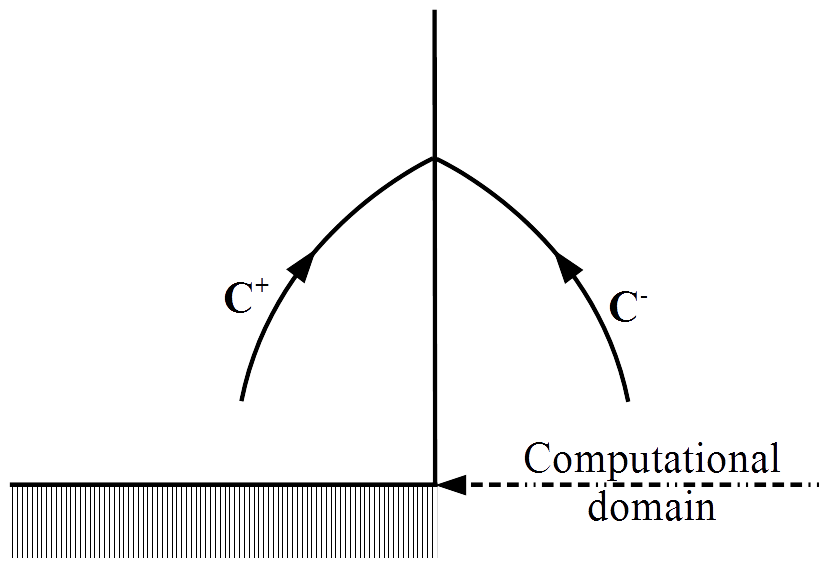
\includegraphics[width=0.8\textwidth]{Figures/AmontFluvial.png}
  \caption{Upstream subcritical flow}
 \end{center}
\end{figure}

Only one of the characteristics comes from outside the domain. The other characteristic (characteristic $C^-$ in this case) comes from inside the domain and carries information to the boundary of the domain. It is therefore necessary to impose the elevation or the flow but not both variables.

\textbf{B) \underline{Upstream supercritical flow}}

\begin{figure}[H]
 \begin{center}
  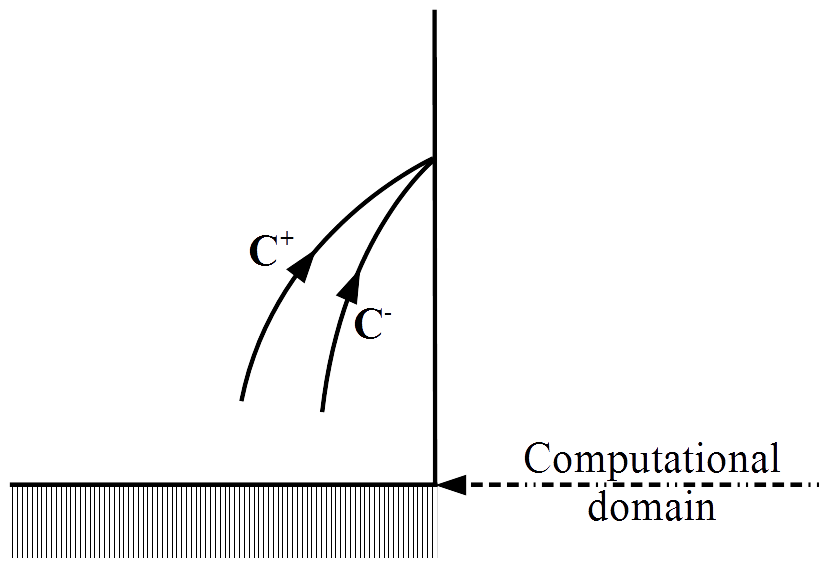
\includegraphics[width=0.8\textwidth]{Figures/AmontTorrentiel.png}
  \caption{Upstream supercritical flow}
 \end{center}
\end{figure}

Both characteristics come from outside the domain. In this case it is necessary to impose the elevation and the flow.

\textbf{C) \underline{Downstream subcritical flow}}

\begin{figure}[H]
 \begin{center}
  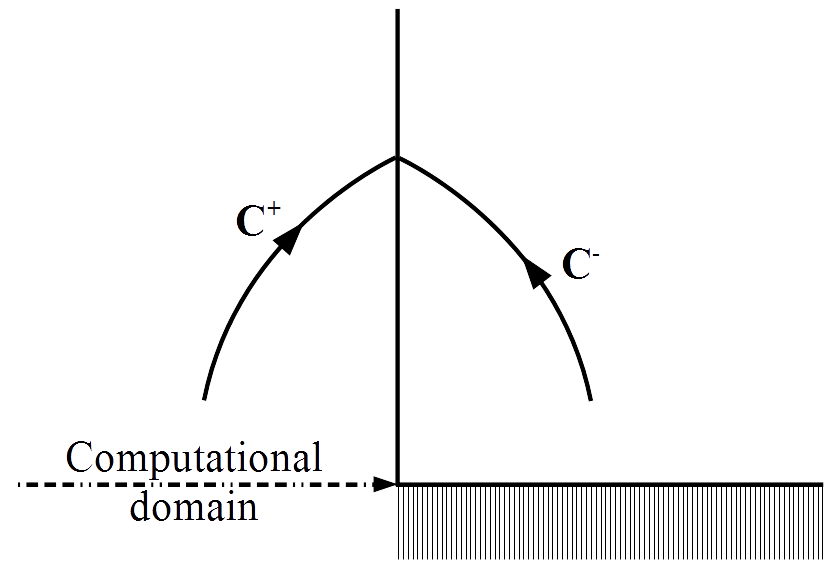
\includegraphics[width=0.8\textwidth]{Figures/AvalFluvial.png}
  \caption{Downstream subcritical flow}
 \end{center}
\end{figure}

These are the same conditions as for upstream subcritical flow. Only one of the variables therefore has to be imposed (either the elevation or the flow). In practice, the elevation is often chosen.

\textbf{D) \underline{Downstream supercritical flow}}

\begin{figure}[H]
 \begin{center}
  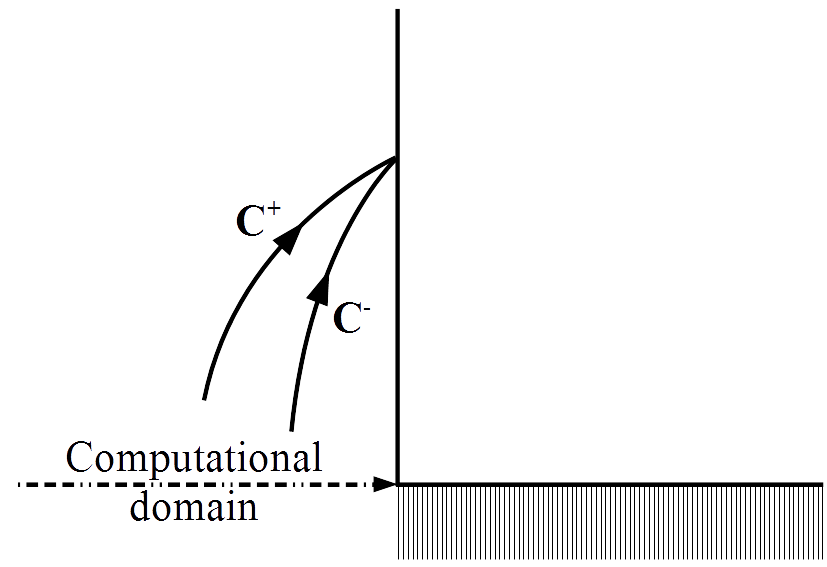
\includegraphics[width=0.8\textwidth]{Figures/AvalTorrentiel.png}
  \caption{Downstream supercritical flow}
 \end{center}
\end{figure}

Both characteristics come from inside the domain. No extra information is required.

The following table summarises the scenarios described above.

\begin{table}[h]
\centering
\caption{Type of flow and upstream/downstream boundary conditions}
\begin{tabular}{c|c|c}
  &\textbf{Subcritical} & \textbf{Supercritical} \\
  \hline
  Upstream & Elevation or Flow & Elevation \textbf{and} Flow \\
  Downstream & Elevation or Flow & nothing \\
  \hline
 \end{tabular}
 \label{TabCL}
\end{table}

%...............................................................................
\subsubsection{Modelling the boundary conditions}
%...............................................................................

The numerical scheme defined in section \ref{PbHom} assumes that the values for the two variables are known at every time step at the boundary of the domain. This, however, can be conflicting with the scenarios introduced in the previous section and following from the characteristics method.

Initially, it is assumed that the boundary conditions are entirely known. The following will focus on how they are taken into account in the overall scheme.

Let us consider a given flow rate applied upstream of the domain.

\begin{figure}[H]
 \begin{center}
  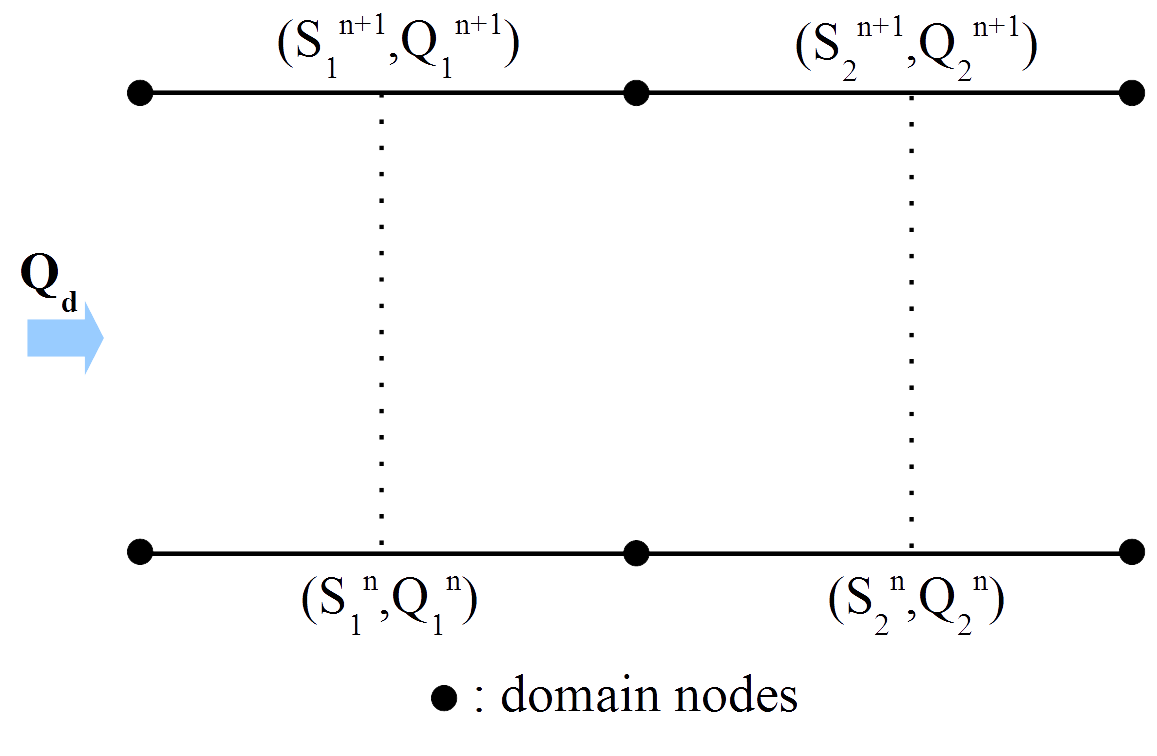
\includegraphics[width=0.8\textwidth]{Figures/NDomaine.png}
  \caption{Downstream supercritical flow}
 \end{center}
\end{figure}

Let us suppose that all the variables are known at the time step $n$.

All the variables at all the nodes in the domain, except those at the boundary, can be evaluated at the time step $n+1$ with the Roe scheme. There are two options to compute $(S_{1}^{n+1},Q_{1}^{n+1})$ :
\begin{itemize}
 \item $(S_{1}^{n+1},Q_{1}^{n+1})$ is computed using the Roe scheme, where the conditions to the left are given by the boundary conditions $(Q_r,S_r)$. It is important to note that the wetted cross-section $S_r$ is not provided by the user but is computed. The following section will introduce how the missing information can be computed;
 \item the first half of the cell is not considered as a cell in the finite volume definition. $(S_{1}^{n+1},Q_{1}^{n+1})$ is set to be equal to the boundary condition $(Q_r,S_r)$. As was the case before, the wetted cross-section will be computed separately.
\end{itemize}

The second method was selected to treat the boundary conditions since it guarantees that the values imposed by the user are found at the first mesh node. This is not guaranteed with the first method.

The various methods available in \mascaret{} to calculate the boundary condition information, independently from the finite volume scheme, are presented in the following sections.

\textbf{A) \underline{Computation of the boundary conditions using the Riemann invariants}}

The principle of this method is very simple and based on the non-\linebreak conservative form of the Saint-Venant equations. It is based on the assumption that the solution is continuous in the immediate vicinity of the boundary conditions. Four possible scenarios can be identified (refer to table \ref{TabCL}) depending on the nature of the flow and on whether considering the upstream or downstream sections.

$\Longrightarrow$ \textsc{Upstream boundary of the domain}

$\rightarrow$ Supercritical flow

The two characteristics enter the domain: it is therefore necessary to provide both the value of the wetted cross-section and that of the flow.

$\rightarrow$ Subcritical flow

The characteristic $C^-$ leaves the domain and carries information from inside the domain towards the upstream boundary condition. This information, the Riemann invariant $f^-$, will be used to supplement the data (wetted cross-section or flow) that the user will have to provide.

This computation is detailed as follows.

$Q_1^{n+1}$ or $S_1^{n+1}$, which are known (provided as input), give a first relationship.

The Riemann invariant $f_{1}^+$ is constant along the characteristic curve $C^-$ resulting from the upstream boundary of the model. This yields a second relationship.

The following system is to be solved :

\begin{equation}
 \left \lbrace
  \begin{array}{l}
    Q_{1}^{n+1} \quad \mbox{or} \quad S_{1}^{n+1} \quad \mbox{known} \\
    \\
    \frac{Q_{1}^{n+1}}{S_{1}^{n+1}} + K(S_{1}^{n+1}) = f_{1}^+
  \end{array}
 \right.
\end{equation}

\begin{itemize}
 \item Imposed flow : the second equation is multiplied by $S_{1}^{n+1}$ to determine $S_{1}^{n+1}$, giving :
   \begin{equation}
     S_{1}^{n+1} K(S_{1}^{n+1}) - f_{1}^+ S_{1}^{n+1} + Q_{1}^{n+1} = 0
   \end{equation}
   This last equation is solved using a Newton method.
 \item Imposed elevation : the computation is much simpler.
   \begin{equation}
      Q_{1}^{n+1} = -S_{1}^{n+1} K(S_{1}^{n+1}) + f_{1}^+ S_{1}^{n+1}
   \end{equation}
\end{itemize}

$\Longrightarrow$ \textsc{Downstream boundary of the domain}

$\rightarrow$ Supercritical flow

Both characteristics leave the domain. No additional information is therefore necessary. The following system is solved :

\begin{equation}
 \left \lbrace
  \begin{array}{l}
    \frac{Q_{N}^{n+1}}{S_{N}^{n+1}} + K(S_{N}^{n+1}) = f_{N}^+ \quad \mbox{with } f_{N}^+ \mbox{ known} \\
    \\
    \frac{Q_{N}^{n+1}}{S_{N}^{n+1}} - K(S_{N}^{n+1}) = f_{N}^- \quad \mbox{with } f_{N}^- \mbox{ known}
  \end{array}
 \right.
\end{equation}

$\rightarrow$ Subcritical flow

This is similar to the upstream subcritical flow scenario.

\begin{CommentBlock}{Note :}
The computation of the boundary conditions using the Riemann invariants is satisfactory and respects the theory of the characteristics. Studies have, however, indicated that this method gives significant errors in cases of small Froude number flows. This is attributed to the fact that the dominant term in the equation is then $SK(S)$ where $K(S)$ is a non-linear function which had to be tabulated (vertical discretisation). To mitigate this major shortcoming for subcritical flows, other methods have been introduced, which are based on a finite difference discretisation of the continuity or momentum equations.
\end{CommentBlock}

\textbf{B) \underline{Computation of the boundary conditions using the Saint-Venant equations}}

This is only relevant for subcritical flows.

$\Longrightarrow$ \textsc{Upstream boundary of the domain}

\begin{itemize}
 \item Imposed flow : the continuity equation is discretised in the simplest possible way using finite differences, to give :
   \begin{equation}
     Q_{1}^{n+1} = Q_r
   \end{equation}
   and :
   \begin{equation}
     \frac{S_{1}^{n+1}-S_{1}^{n}}{\Delta t} + \frac{Q_{2}^n - Q_{1}^n}{\Delta x} = 0
   \end{equation}
   $S_{1}^{n+1}$ is computed using the previous equation.
 \item Imposed elevation : the momentum equation is discretised in a similar way to that used to discretise the continuity equation.
\end{itemize}

$\Longrightarrow$ \textsc{Downstream boundary of the domain}

There is no added difficulty in this case. The approach is similar.

A parameter, called \textit{limit Froude}, which is imposed by the user (refer to user manual) determines the choice of the method to compute the boundary conditions. If the Froude number, upstream or downstream of the domain, is greater than this parameter, the missing information for the boundary conditions will be computed using the Riemann invariants.

\textbf{C) \underline{Representation of a stage-discharge curve}}

So far only the simplest cases have been considered where the elevation or the flow is imposed. For real applications, however, a very useful boundary condition is a \textit{stage-discharge curve} : the elevation and the flow are not known explicitly but are interlinked with a relationship $Z = f(Q)$. The system with two equations and two unknowns is solved to obtain the value of the flow and of the elevation at the domain boundaries. The only difference with the previous cases is that the first equation is not straightforward any more.

\textbf{D) \underline{Representation of a free downstream flow}}

The methods introduced in the previous sections make it possible to compute missing information in the case of subcritical flows but it is still necessary to provide at least the elevation or the flow. This is difficult for flood wave computations where it is impossible for the user to know the elevation or the flow at the downstream boundary of the domain. To address this, it was tried to represent a \textit{free downstream flow}. In this case the user does not provide any boundary condition, these are computed using values from the previous time step only. It is clear that this representation is not correct in consideration of the characteristics method applied to the Saint-Venant equations. The purpose of this representation is not to provide a correct flow for the boundary condition but to let the flood wave leave the domain without influencing too much the flow within the domain.

To obtain a \textit{free downstream flow}, the two variables wetted cross-section and flow rate are moved along at the flow speed.

For flood wave computations it is recommended that the downstream boundary condition for the computational domain is located at least 30 km downstream of the last computational point in order not to disrupt the characteristics at this point. It is strongly advised not to use this type of boundary condition for any other type of computation.

%...............................................................................
\subsection{Dry areas}
%...............................................................................

For applications such as flood waves, it is necessary to be able to model dry areas and the propagation of a front on dry areas. From a numerical viewpoint, the following problems arise :
\begin{itemize}
 \item definition of a flow regime in the dry area because speed is not defined;
 \item propagation of a front on dry areas.
\end{itemize}

The main objective with this problem is to calculate a good propagation velocity of the front since this information is paramount to flood wave computations.

To treat this problem with the Roe scheme, a threshold had to be introduced for the water depth. Using this approach the correct propagation velocity was found on simple test cases where an analytical solution exists \cite{GOUTAL97}. The drawback with this approach is that the perfect conservativity inherent to the finite volumes is then lost. For flood wave computations, the Roe scheme was retained but this entails a strict control of the conservativity.

It should be noted that, within the IAHR work group on numerical methods for flood waves on dry ground, all the teams face the same difficulties.
One of the only schemes that does not have this problem is the so-called equilibrium scheme, developed at the university of Bordeaux by Professor Leroux's team \cite{LECOZ96}\cite{BON97}.

It will be necessary to consider other approaches than that of the threshold depth in the future, but it is a satisfactory solution in the meantime.

%-------------------------------------------------------------------------------
\section{Representation of more complex physical phenomena}
\label{ModelCplx}
%-------------------------------------------------------------------------------

%...............................................................................
\subsection{Introduction to the modelling of compound channels}
%...............................................................................

The transcritical engine of \mascaret{} treats flows in compound channels made up of a low flow channel (river bed) and a high flow channel (floodplain), but storage zones are not considered.

\begin{figure}[H]
 \begin{center}
  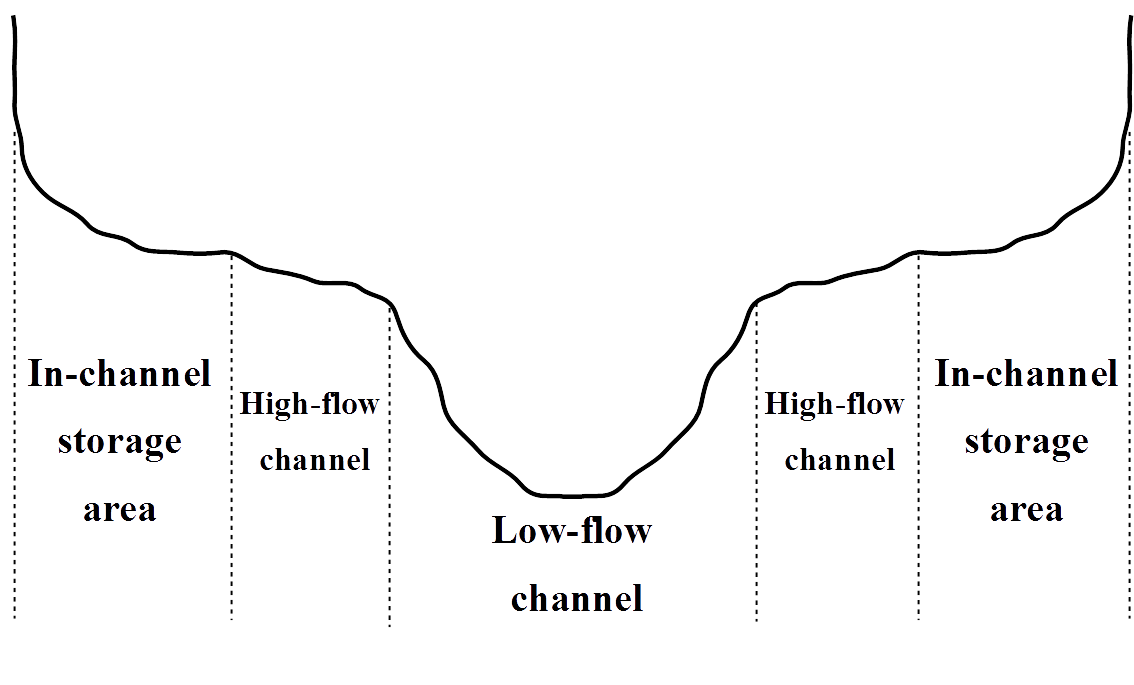
\includegraphics[width=\textwidth]{Figures/Lits.png}
  \caption{Channels and storage sections}
 \end{center}
\end{figure}

The \emph{Debord} formulation was selected to model the low flow and high flow channels such that the subcritical and transcritical engines are as much compatible as possible.

%...............................................................................
\subsubsection{Reminder}
%...............................................................................

The system of equations to solve can now be written as :

\begin{equation}
 \label{SyEQ}
 \left \lbrace
  \begin{array}{l}
    \frac{\partial S}{\partial t} + \frac{\partial Q}{\partial x} = q_l - \frac{\partial S_s}{\partial t} \\
    \\
    \frac{\partial Q}{\partial t} + \frac{\partial}{\partial x} \left ( \frac{Q_{m}^2}{S_m} + \frac{Q_{M}^2}{S_M} + P \right ) \\
    \\
    \quad = g \int_{0}^y \left ( \frac{\partial S}{\partial x}\right )_y \, dy - g S \frac{d Z_f}{d x} - g (S_m J_m + S_M J_M)
  \end{array}
 \right.
\end{equation}

with :

\begin{itemize}
 \item $q_l$ the inflow and $S_s$ the storage section;
 \item $S = S_m + S_M$ and $Q = Q_m + Q_M$;
 \item $\sqrt{J_m} = \frac{Q_m}{D_m}$ and $\sqrt{J_M} = \frac{Q_M}{D_M}$;
 \item $D_m = K_m S_m R_{m}^{2/3}$ and $D_M = K_M S_M R_{M}^{2/3}$ are the conveyances in the river bed and in the floodplain respectively, and depend on the free surface elevation.
\end{itemize}

This system is similar to the Saint-Venant equations in the case of a single channel with the overall slope $J$ defined by means of the relation :

\begin{equation}
 S J = S_m J_m + S_M J_M
\end{equation}

and with the $\beta$ coefficient no longer equal to 1 (as in a river bed), but satisfying the relation :

\begin{equation}
 \beta \frac{Q^2}{S} = \frac{Q_{m}^2}{S_m} + \frac{Q_{M}^2}{S_M}
\end{equation}

\begin{CommentBlock}{Note :}
the $\beta$ coefficient is greater than or equal to 1.
\end{CommentBlock}

%...............................................................................
\subsubsection{The \emph{Debord} formulation}
%...............................................................................

The system of equations (\ref{SyEQ}) is not complete and a closing relation is necessary. Various solutions have been proposed to represent the composition of the two channels. The \emph{Debord} formulation was eventually retained to be compatible with the subcritical engine (refer to section \ref{ModDeb}) and following feedback from various applications of this formulation.

Given :

\begin{equation}
 \eta = \frac{Q_m}{Q_M}
\end{equation}

With the \emph{Debord} formulation :

\begin{equation}
 \eta = \frac{A}{\displaystyle \sqrt{1+\frac{S_m}{S_M}}(1-A^2)} \frac{D_m}{D_M}
\end{equation}

where $A$ is a constant of the \emph{Debord} formulation, computed with :

\begin{equation}
 \left \lbrace
  \begin{array}{l}
    A = \frac{1-A_0}{2}\cos \left ( \frac{\pi r}{0.3} \right ) + \frac{1+A_0}{2} \quad \mbox{for } r=\frac{R_M}{R_m} \in [0,0.3] \\
    \\
    A = A_0 = 0.9 \left ( \frac{K_m}{K_M} \right )^{-1/6} \quad \mbox{for } r > 0.3
  \end{array}
 \right.
\end{equation}

%...............................................................................
\subsubsection{Implementation in the transcritical engine}
%...............................................................................

The equations for compound channels only differ from those for single channels by the $\beta$ term and the form of the source term related to friction. The resolution of this system is therefore formally identical to that treated previously.

The \emph{Debord} formulation makes it possible to write $\beta$ in the form $\beta(S,x)$. This gives an additional unknown function.

For simplicity, the $\beta$ function will be taken into account explicitly. The momentum equation to be solved at time $n+1$ is therefore :

\begin{equation}
 \frac{\partial Q}{\partial t} + \frac{\partial}{\partial x} \left ( \beta^n \frac{Q^2}{S} + P \right ) = g \int_{0}^y \left ( \frac{\partial S}{\partial x} \right )_y \, dy - g S \frac{d Z_f}{dx} -g S J
\end{equation}

It is a partial derivative equation for which the $\beta$ coefficient is variable in time.

The advection system is unconditionally hyperbolic because $\beta$ is greater than or equal to 1. The Riemann problem is solved in a similar way to that related to the Saint-Venant equations for a single channel; the eigenvalues for the system are modified. They become : $\beta u + c'$ and $\beta u - c'$ with : $c' = \sqrt{\frac{\partial P}{\partial S} + u^2(\beta^2 - \beta)}$. The Roe variables remain unchanged.

The representation of friction in this case is exactly identical to that in the case of a single channel; the generalised conveyance takes into account both the river bed and the floodplain, and can be discretised along the vertical in a similar way to the conveyance of the low flow channel.

\begin{CommentBlock}{Note 1 :}
The fact that the $\beta$ term is considered as a forcing function, varying with each time step, simplifies considerably the implementation of the method. This assumption is partly justified because flows in compound channels are generally evolving slowly.
\end{CommentBlock}

\begin{CommentBlock}{Note 2 :}
Conservation properties are lost when modelling compound channels. These properties made it possible to reach a steady state with constant flow. In all the cases studied to date, variations in the flow of the order of $2$ to $3\%$ of the total flow have been observed when a stationary state is reached.
\end{CommentBlock}

%...............................................................................
\subsection{Confluence}
%...............................................................................

A new method has been developed to model confluences. A detailed description can be found in document \cite{MAUREL96} together with validation test cases. The following paragraph summarises the method.

It can be assumed that the 2D Saint-Venant equations replace the 1D equations to represent the flow locally, at and around the junction. It can then be considered that the total domain (main valley + tributary) is the overlap of two sub-domains, where the first sub-domain consists in three 1D reaches (the one-dimensional Saint-Venant equations are supposed to be valid in this case) and where the second sub-domain is the zone around the junction (the two-dimensional equations are supposed to be valid in that case). Modelling the confluence therefore amounts to performing a 1D-2D coupling between the two sub-domains. The 2D Saint-Venant equations are solved using a finite volume module equivalent to that used in 1D (Roe scheme). This module has numerical schemes similar to those used in \mascaret{}. This last point together with the fact that such schemes are explicit has the advantage of facilitating the coupling procedure.

A two-dimensional model usually requires a fine discretisation of the geometry. For flood wave studies, it would not be practical to create a local 2D model for every tributary in a valley, with detailed representation of the geometry and a fine mesh. A simple tool that automate this process is considered as the best approach.
This is why it was decided that the one-dimensional software generates automatically the 2D domain representative of the confluence and the associated mesh. A 12 cells mesh is created by default.

\begin{figure}[H]
 \begin{center}
  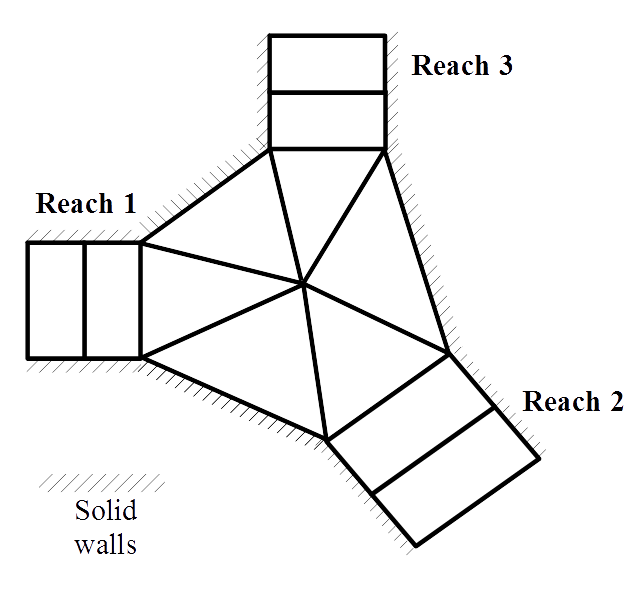
\includegraphics[width=0.8\textwidth]{Figures/ConfPar.png}
  \caption{2D confluence}
 \end{center}
\end{figure}

%...............................................................................
\subsubsection{1D-2D coupling}
%...............................................................................

In the one-dimensional model, the aim is to compute the value of $(S_1,Q_1)$ at the boundary of each 1D reach linked to the confluence. This is equivalent to defining the 1D-2D coupling.

The coupling is done by overlapping domains, i.e. the boundary points of the 2D model are located inside the 1D model. For illustrative purposes, the following figure shows the overlap between the 2D model and the three 1D reaches.

It is assumed that the boundaries of the 1D model, where reaches $B_1$, $B_2$, $B_3$ are located, are represented in the 2D model by cells $A$, $B$, $C$ respectively. Cells $a$, $b$, $c$, at the boundaries of the 2D model, represent the cells close to the ends to each 1D reach. The 1D-2D coupling is then done by exchange of boundary conditions.

\begin{figure}[H]
 \begin{center}
  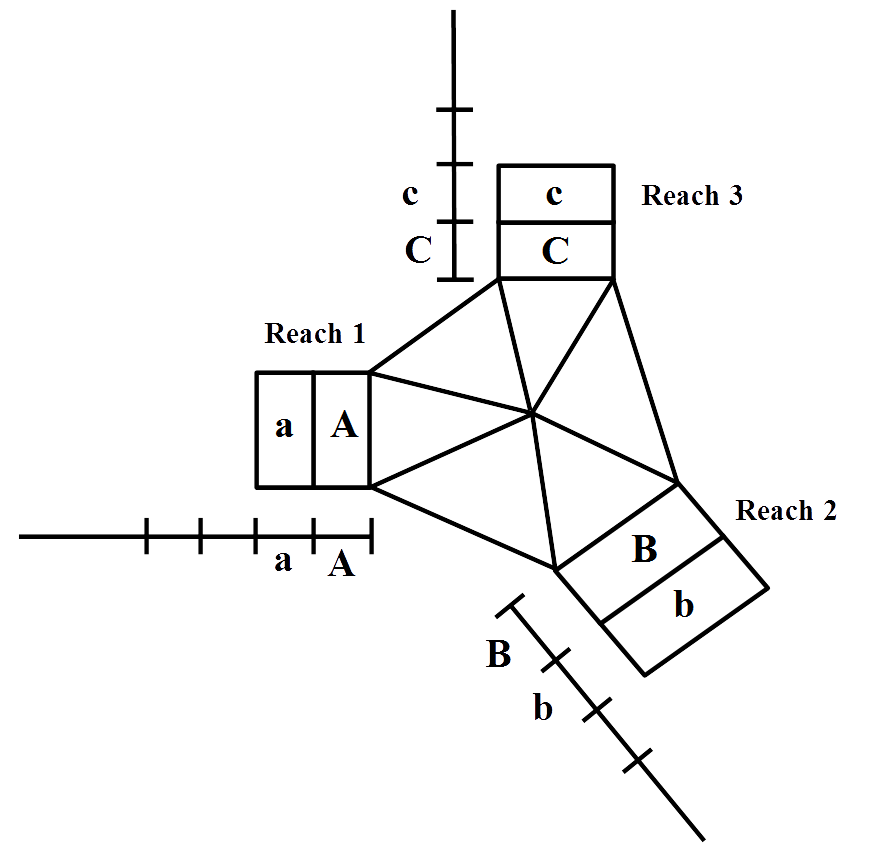
\includegraphics[width=0.8\textwidth]{Figures/ConfPar2.png}
  \caption{1D-2D overlap}
 \end{center}
\end{figure}

A computation can be described as follows :

The state in each 1D reach: $B_1$, $B_2$, $B_3$ and in the 2D confluence is assumed to be known at time $n$. The state at time $n+1$ is determined in four steps :
\begin{itemize}
 \item \textbf{Step 1 :} computation of the state at the confluence (except for the three boundary cells $a$, $b$ and $c$). This stage is carried out with a 2D Roe scheme. The scheme is explicit; the boundary conditions at time $n+1$ are not required, only the conditions for state $n$ everywhere;
 \item \textbf{Step 2 :} computation of the state inside each reach (except for boundary cells $A$, $B$, $C$). This stage is carried out with a 1D Roe scheme for the same reasons and in the same way as previously discussed;
 \item \textbf{Step 3 :} computation of $S_1$, $Q_1$ in each reach. These are the values of $S$ and $Q$ in $A$, $B$, $C$. These values have been computed at step 1. The free surface level is maintained from one model to the other. The computed flow values, however, are two-dimensional. The flow vector is therefore projected along the normal to the free boundary in order to obtain a one-dimensional value.
 \item \textbf{Step 4 :} computation of the boundary conditions for the 2D model. These were determined at step 2 in the cells adjacent to the ends of each reach. Similarly to the previous step, the free surface level is maintained from the 1D model to the 2D model. Furthermore, the flow direction is assumed to be that of the normal to the free boundary in order to have a two-dimensional flow.
\end{itemize}

Finally, the complete state of the one-dimensional model (reaches $B_1$, $B_2$, $B_3$) and of the two-dimensional model (the confluence) is computed at time $n+1$.

The use of a finite volume scheme in the 2D model makes modelling of the confluence a priori conservative. This is not entirely true because a projection of the flow is used to go from the 2D state to the 1D state and this introduces a source of non-conservatism to the momentum.

%...............................................................................
\subsubsection{Adapting the 1D geometry to the 2D model}
%...............................................................................

Now that the coupling method has been defined, all that remains is to describe the 2D model selected to represent the junction. Initially, the simple case of rectangular channels is considered. Then the method is extended to real geometries.

$\Longrightarrow$ Rectangular channels

The geometry of the junction is discretised using twelve cells such that it is reasonnable close to the real geometry.

\begin{itemize}
 \item[*] For each tributary, the coordinates of the boundary point on the hydraulic axis are provided, as well as the angle this 1D reach forms with a set direction. These are the only external data specific to the confluence. They are determined only from geometrical criteria;
  \begin{figure}[H]
    \begin{center}
     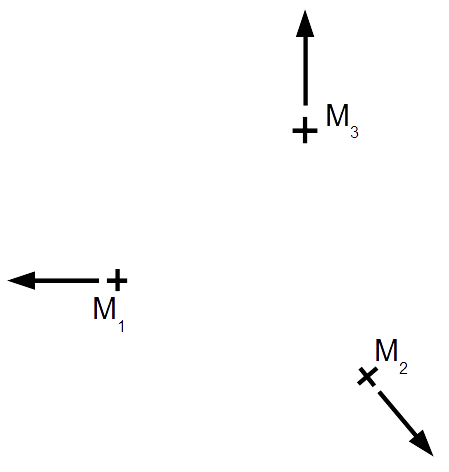
\includegraphics[width=0.5\textwidth]{Figures/cr1.png}
    \end{center}
  \end{figure}

 \item[*] for each tributary $i$, a segment can be traced with length $L_i$ (the width of the channel, independent from the definition of the confluence, and coming directly from the geometry of the 1D model). This segment is normal to the angle previously set;
  \begin{figure}[H]
    \begin{center}
     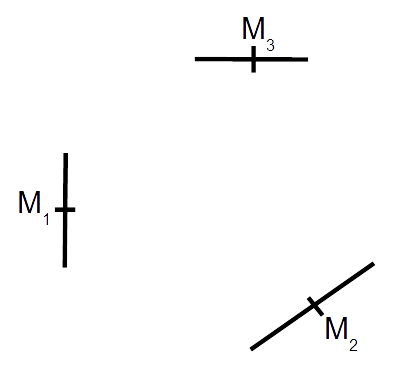
\includegraphics[width=0.5\textwidth]{Figures/cr2.png}
    \end{center}
  \end{figure}

 \item[*] these segments are then joined up by walls. The three segments previously defined together with the walls form a hexagon at the junction;
   \begin{figure}[H]
    \begin{center}
     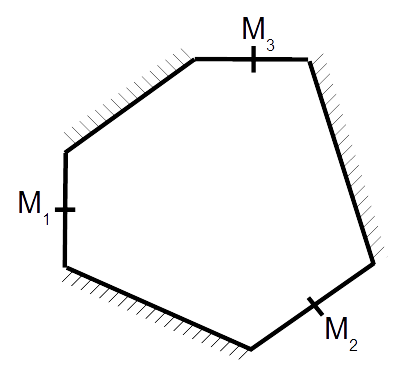
\includegraphics[width=0.5\textwidth]{Figures/cr3.png}
    \end{center}
  \end{figure}

 \item[*] $G$ is the centre of gravity of the hexagon. Inside the hexagon, six triangles are formed with $G$ as a common vertex;
  \begin{figure}[H]
    \begin{center}
     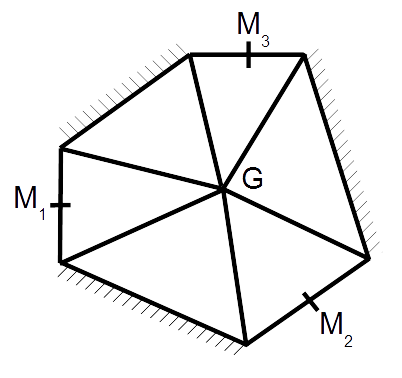
\includegraphics[width=0.5\textwidth]{Figures/cr4.png}
    \end{center}
  \end{figure}

 \item[*] the cells in the 1D-2D overlapping area are rectangles with sides $L_i$ and $DX_i$, the size of the 1D cell in each reach;
  \begin{figure}[H]
    \begin{center}
     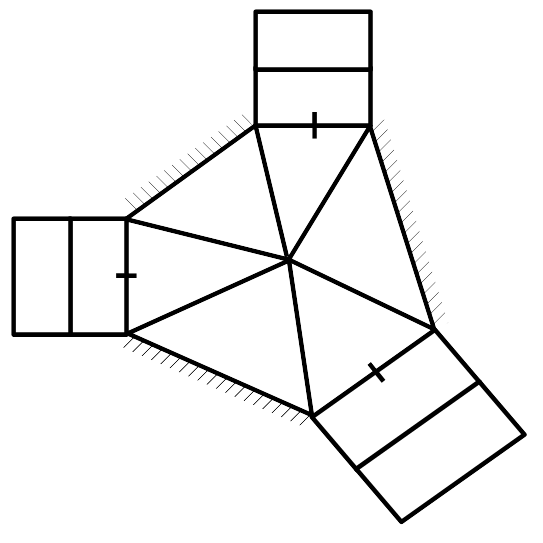
\includegraphics[width=0.5\textwidth]{Figures/cr5.png}
    \end{center}
  \end{figure}

 \item[*] last but not least, the bottom elevation in each cell is set as follows :
   \begin{itemize}
     \item for the six overlapping cells, it is the elevation of the 1D cell, $Z_{f1D}$;
     \item inside the hexagon, the elevation of $G$ ($Z_{fG}$) is taken to be the arithmetic mean of those in the three neighbouring 1D-2D overlapping cells. The three cells that have an edge in common with the overlapping cells (thus no walls) have an elevation $Z_{f2D}$ defined by : $Z_{f2D} = \frac{2Z_{f1D}+Z_{fG}}{3}$ where $Z_{f1D}$ is the elevation of the adjacent 1D cell;
     \item for each of the other three cells, the bottom elevation is assumed to be the average of the elevation at the two adjacent cells.
   \end{itemize}
\end{itemize}

This parameterisation has the advantage that it only requires few specific parameters: the coordinates of points $M_i$ and the relative orientation of each reach. These are purely geometrical parameters, which are easy to determine. The remainder of the information comes directly from the 1D parameterisation (geometry of the cross-reach profiles) and from the state of each reach.

The geometry thus defined takes into account :

\begin{itemize}
 \item the importance of the extent of the zone of confluence, through the relative position of the three points $M_i$;
 \item the orientation of each reach, through the angles provided for each $M_i$;
 \item the width of each channel, since it is transferred in the 2D model from the 1D state;
 \item the bottom variations, since the elevation of the overlapping cells is that of the 1D cells. Inside the hexagon, the bottom elevations vary smoothly.
\end{itemize}

$\Longrightarrow$ Real geometry channels

A difficulty arises in the case of a real geometry. A cross-section will be discretised using only one cell in the 2D model. This 2D cell represents a rectangular profile since the bottom of a cell is flat with the $P_0$ discretisation used here. This point was obviously trivial in the previous case, but must now be addressed specifically.

The problem is to find the rectangular geometry equivalent to the real geometry, in the sense that the flows represented in each model must be as close as possible. A 1D-2D transformation must therefore be defined and the following was retained :
\begin{itemize}
 \item the bottom elevation $Z_f$ is preserved;
 \item the free surface elevation $Z$ is preserved (thus $Y$, the water depth, is also preserved);
 \item the discharge $Q$ is preserved;
 \item the velocity $V$ is preserved.
\end{itemize}

It is thus necessary to preserve the wetted cross-section $S$. The depth being fixed by the first two points, the width can be deduced from :

\begin{equation}
 L_{2D} = \frac{S_{1D}}{Y}
\end{equation}

This cell width is likely to change when the depth varies. The grid must therefore be updated in a regular way at each time step.

%...............................................................................
\subsection{Singularities}
%...............................................................................

When a flood wave propagates in a real valley, dams located downstream of the main dam need to be taken into account. These structures can respond in several possible ways: instantaneous failure when the wave arrives or spilling over the crest of the structure. In the second case, the dam can be modelled in two different ways :

\begin{itemize}
 \item direct representation in the geometry. This solution, however, would require a very fine grid in the immediate proximity of the structure since the slopes of the faces are steep upstream and downstream of the structure. This would strongly constrain the time step for the whole computational domain;
 \item representation as a singularity. With this option the dam is not treated as a regular node in the numerical scheme. Instead, a specific relationship relates the water upstream and downstream of the dam.
\end{itemize}

The method used to model a singularity in the case of a finite volume scheme will be introduced in the remainder of this section.

It is considered that a singularity is defined by a relation linking the conveying flow $Q_s$ through this singularity to the upstream and downstream water levels. This relation depends on the physical and hydraulic characteristics of the structure.

A part of the domain is represented in the figure below.

A singularity has to be located at the interface between 2 cells. The flow through this interface is defined by : $Q_s = f(Z_{i-1},Z_i)$.

\begin{figure}[H]
    \begin{center}
     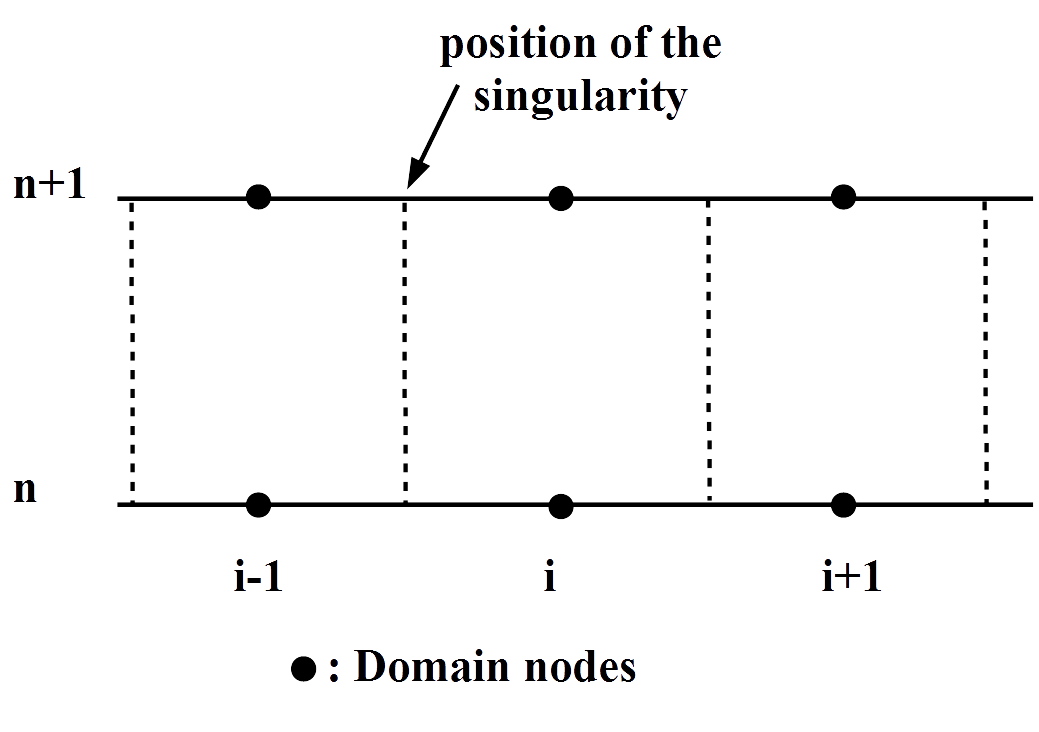
\includegraphics[width=0.8\textwidth]{Figures/posSing.png}
    \end{center}
\end{figure}

With a finite volume scheme, the hydraulic state in cells $i$ and $i-1$ at time $n+1$ depends on the fluxes at the interface of both cells.

For cell $i$ (respectively $i-1$), the flux to the right (respectively to the left) will be that computed by the scheme defined in section $n$. The mass and momentum fluxes at the interface between cell $i$ and cell $i-1$, however, will not be that of Roe, but the analytical flux explicitly computed using the relation defining the singularity.

\textbf{\underline{For cell $i$}}

Mass flux to the left : $Q_s =f(Z_{i-1}^n,Z_{i}^n)$

Momentum flux to the left : $\frac{Q_{s}^2}{S_{i}^n} + P(S_{i}^n)$

\textbf{\underline{For cell $i-1$}}

Mass flux to the right : $Q_s =f(Z_{i-1}^n,Z_{i}^n)$

Momentum flux to the right : $\frac{Q_{s}^2}{S_{i-1}^n} + P(S_{i-1}^n)$

\begin{CommentBlock}{Note :}
\begin{itemize}
 \item mass is therefore conserved. Momentum, however, is no longer conserved;
 \item at the very beginning of the spill, the wetted cross-section downstream of the singularity is very small. This implies very strong flows and consequently numerical problems (instabilities). In this situation, only the pressure term is kept in the momentum flux equation;
 \item this representation allows all types of singularities to be taken into account. All that is required is the function linking the discharge to the upstream and downstream elevations.
\end{itemize}
\end{CommentBlock}

%...............................................................................
\subsection{Eroding dams}
%...............................................................................

The transcritical engine of \mascaret{} makes it possible to model erosion, by overflow, of the gravity dams located downstream of the principal dam.

The selected method is largely inspired from that implemented in the \texttt{EROSIF} solver \cite{BENSLAMA95}. \texttt{EROSIF} computes the evolution of a breach in an embankment as well as the downstream hydrograph resulting from the progressive failure.

Within \mascaret{}, a dam eroding by overflow is treated as a spilling dam with a crest elevation variable in time.

\begin{figure}[H]
    \begin{center}
     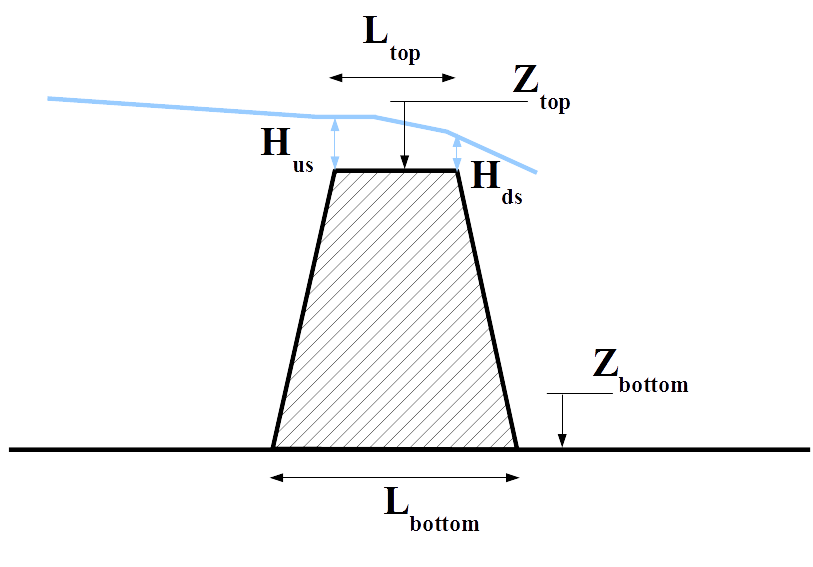
\includegraphics[width=0.8\textwidth]{Figures/BarPds.png}
     \caption{Modelling notations}
    \end{center}
\end{figure}

Upstream of the dam, the hydraulic conditions are assumed to be identical to those computed by the transcritical engine in the cell immediately upstream of the dam at the previous time step.

Downstream of the dam, a critical condition is imposed. The flow across the whole structure is assumed to be equal to the upstream flow.

The evolution of the elevation of the dam crest is given by the equation :

\begin{equation}
 (1-p) \frac{dZ_{top}}{dt} = - \frac{dQ_s}{dx} = - \frac{Q_{s_{d/s}}-Q_{s_{u/s}}}{L_{top}}
\end{equation}

where $p$ is the porosity of the material (usually taken as 0.4), $Q_{s_{u/s}}$ et $Q_{s_{d/s}}$ are the sediment transport rate respectively upstream and downstream of the erosion channel, and calculated using the of Meyer Peter Muller formulation, i.e. :

\begin{equation}
 Q_s = \frac{8}{g \sqrt{\rho}(\rho_s - \rho)}(\tau - \tau_c)^{1.5}
\end{equation}

with :
\begin{itemize}
 \item $\tau$ the global hydrodynamic stress (Manning Strickler formulation);
 \item $\tau_c$ the critical shear stress : $0.05 . (\rho_s - \rho).g.d_{50}$;
 \item $\rho_s$ the density of the sediment;
 \item $\rho$ the density of water;
 \item $d_{50}$ the median diameter of the material.
\end{itemize}

All these equations make it possible to compute $Z_{top}$, the crest elevation. Erosion is limited at the bottom by the elevation $Z_{low}$.

%...............................................................................
\subsection{Broad-crested and sharp-crested weirs}
\label{LoiSeuilMinceEpais}
%...............................................................................

This section presents the methodology for modelling singularities of the type broad-crested or sharp-crested weirs, as implemented in the transcritical and subcritical engines. For the other singularities, the pair (flow, elevation) is directly determined by interpolation from a discretised table, provided by the user.

The laws for weirs implemented in the transcritical and subcritical engines give the user a choice between two types of weirs: broad-crested or sharp-crested weirs. These two laws differ only when the weir is drowned, in particular with the flow conditions and the drowning coefficient.

The validation tests carried out in the case of a sharp-crested weir are detailed in \cite{GOUTAL03}.

%...............................................................................
\subsubsection{Broad-crested or sharp-crested free flow weir}
%...............................................................................

\begin{figure}[H]
    \begin{center}
     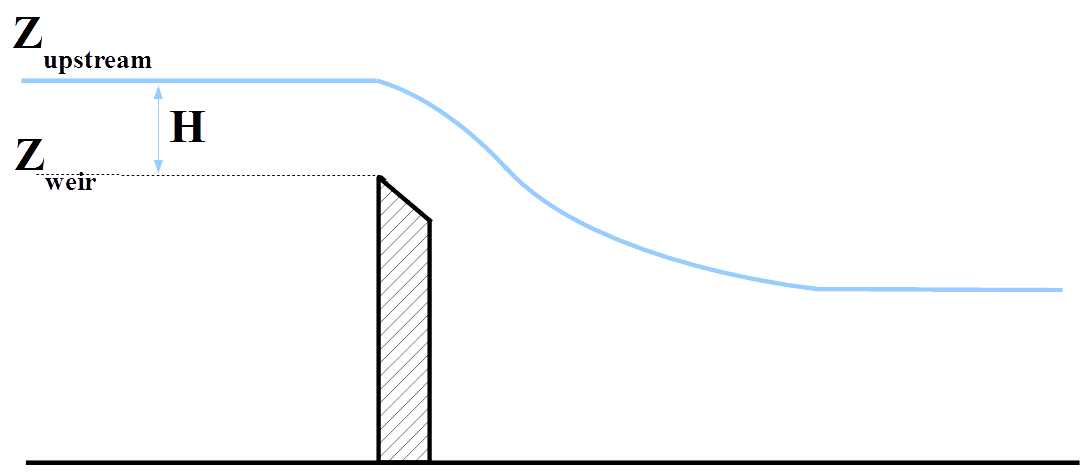
\includegraphics[width=0.8\textwidth]{Figures/Sden.png}
    \end{center}
\end{figure}

The flow over a broad-crested or sharp-crested free flow weir can be expressed as :

\begin{equation}
 \label{debSeuil}
 Q = C L H \sqrt{2 g H}
\end{equation}

where:

\begin{itemize}
 \item $H$ is the water head upstream of the weir (the approach velocity is ignored) : $H = Z_{u/s} - Z_{weir}$;
 \item $g$ is the gravity;
 \item $L$ is the width of the weir;
 \item $C$ is a discharge coefficient which depends on contraction effects and on approximations made when writing the formula (\ref{debSeuil}) : for example the fact that the approach velocity is not accounted for. This coefficient, $C$, is determined by the user and can result from a calibration of the model.
\end{itemize}

More details on how the previous formula was established are given in \cite{CARLIER87}.

The laws are identical when the weirs are not drowned. When they are drowned, however, the laws differ with the type of weir (conditions and drowning coefficient).

%...............................................................................
\subsubsection{Drowned weir}
%...............................................................................

\begin{figure}[H]
    \begin{center}
     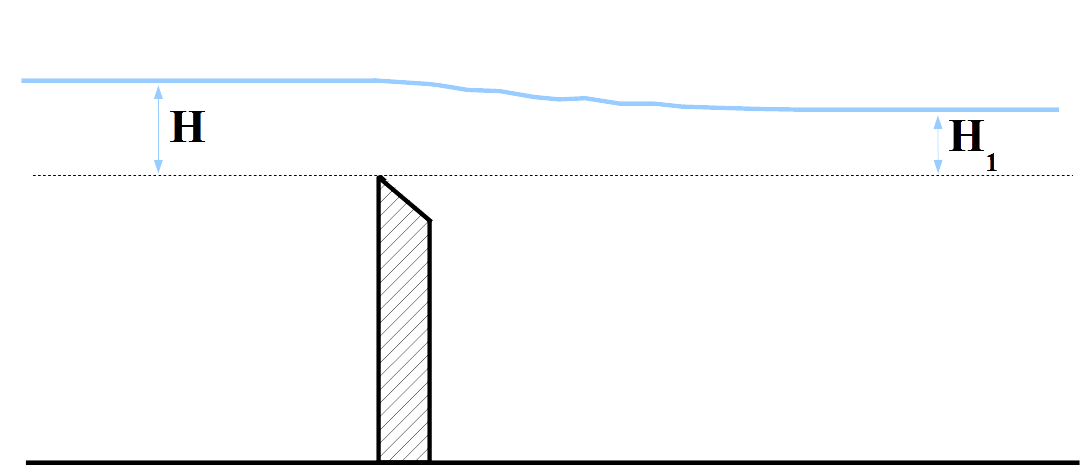
\includegraphics[width=0.8\textwidth]{Figures/Snoy.png}
    \end{center}
\end{figure}

A weir is considered drowned when the upstream elevation is influenced by the downstream elevation. The discharge for a broad-crested or sharp-crested drowned weir can be expressed in a similar way to that for a drowned weir. Only the discharge coefficient, $C$, is modified to take into account the influence of the downstream reach on the discharge over the weir. A drowning coefficient, $K$, is defined as :

\begin{equation}
 K = \frac{Q_{\mbox{drowned flow}}}{Q_{\mbox{free flow}}}
\end{equation}

The discharge over the drowned weir is therefore expressed as :

\begin{equation}
 \label{sny}
 Q = K C L H \sqrt{2 g H}
\end{equation}

where :
\begin{itemize}
 \item $K$ is a coefficient which depends on the ratio $\frac{H_1}{H}$ and the type of weir;
 \item $H=Z_{u/s}-Z_{weir}$ et $H_1 = Z_{d/s}-Z_{weir}$;
 \item $C$ is the discharge coefficient defined above for the drowned weir.
\end{itemize}

$\Longrightarrow$ Broad-crested drowned weir

For a broad-crested weir, the downstream elevation does not influence the discharge over the sill when $H_1$ is lower than $0.8H$ (even though the elevation of the downstream reach may be higher than the weir crest elevation). This is linked to the presence of a critical section over the weir.

The drowning coefficient $K$ in the formula (\ref{sny}) is that typically used for broad-crested weirs. It can be expressed as :

\begin{equation}
 \left \lbrace
  \begin{array}{l}
    K = -25 \left ( \frac{H_1}{H} \right )^2 + 40 \left ( \frac{H_1}{H} \right ) - 15 \quad \mbox{if } \frac{H_1}{H} > 0.8\\
    \\
    K = 1 \quad \mbox{if } \frac{H_1}{H} < 0.8
  \end{array}
 \right.
\end{equation}

$\Longrightarrow$ Sharp-crested drowned weir

For a sharp-crested weir :
\begin{itemize}
 \item if $H_1 < 0$, $K=1$ : the downstream elevation does not influence the discharge over the weir;
 \item if $H_1 > 0$, i.e. as soon as the downstream elevation is higher than that of the weir crest, we have :
   \begin{equation}
     K = \left ( \left ( 1 - \frac{H_1}{H} \right )^{1.5} \right )^{0.385}
   \end{equation}
\end{itemize}

Figure \ref{fig:CFEN} gives the shape of the drowning coefficients as a function of $\frac{H_1}{H}$, for both a broad-crested and a sharp-crested weir.

\begin{figure}[H]
    \begin{center}
     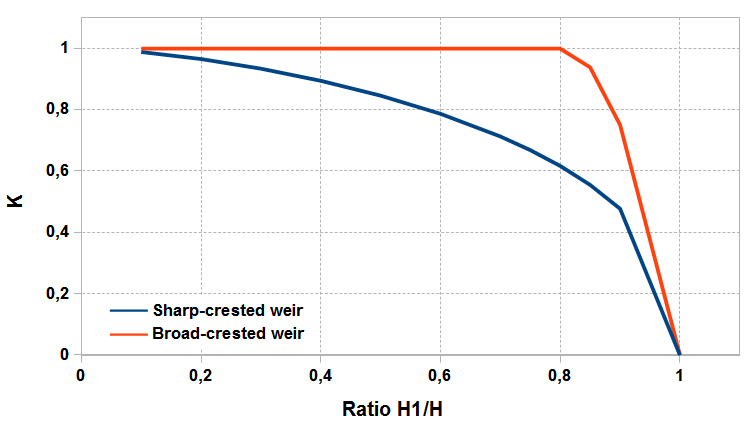
\includegraphics[width=\textwidth]{Figures/CoefEn.png}
     \caption{Drowning coefficient}
     \label{fig:CFEN}
    \end{center}
\end{figure}

%...............................................................................
\subsection{Summary of the treatment of singularities}
\label{BilanSing}
%...............................................................................

There may exist in a river some regions where the Saint-Venant equations do not apply because the assumptions (for example, uniform distribution of the speeds along the vertical) are no longer valid. Flows over weirs, valves etc... are some examples.

The relationships between the elevation and the discharge in the close vicinity of the singularities are then described by explicit laws. The subcritical engines of \mascaret{} can model singularities such as weirs and valves in a river when those are explicitly modelled by hydraulic laws relating the discharge through the singularity, the upstream and downstream elevations and the characteristics of the singularity. Although a number of singularities are implemented in MASCARET, they are not all available for the transcritical engine. The following table lists the various singularities and their availability in the subcritical and transcritical engines.

\begin{table}[H]
\centering
\caption{Singularities modelled in \mascaret{}}
 \label{TBL2}
\begin{tabular}{c|c|c}
  \textbf{Type of singularities} & \textbf{Subcritical engine} & \textbf{Supercritical engine} \\
  \hline
  $Q=f(Z_{d/s})$ & \textbf{yes} & no \\
  $Q=f(Z_{u/s})$ & \textbf{yes} & \textbf{yes} \\
  Law for broad-crested weir & \textbf{yes} & \textbf{yes} \\
  Law for sharp-crested weir & \textbf{yes} & \textbf{yes} \\
  $Z_{u/s}=f(Q)$ & \textbf{yes} & no \\
  $Z_{u/s}=f(Z_{d/s},Q)$ & \textbf{yes} & no \\
  Weir with crest defined by multiple points & \textbf{yes} & no \\
  $Z_{u/s}=f(t)$ & \textbf{yes} & no \\
  Law for valves & \textbf{yes} & no \\
  \hline
 \end{tabular}
\end{table}

%...............................................................................
\subsection{Non-hydrostatic terms}
%...............................................................................

This section presents an extension of the Saint-Venant equations, which considers some of the terms introduced when non-hydrostatic effects are taken into account. The aim is to model physical phenomena such as Favre waves (or undular bores). It should be noted that these developments are only valid for subcritical, unsteady flows with a shallow bed slope. This is derived from work by BRISTEAU et al. \cite{BRISTEAU11}.

The following paragraphs describe the additional terms and their representation within the framework of the transcritical engine in \mascaret{} (finite volume scheme of Roe type). These developments can also be applied without much difficulty to the \REZO{} engine dedicated to subcritical flows. These were the subject of a publication where the reader will find all the necessary explanations \cite{BRISTEAU11}.

The Saint-Venant equations are obtained from the Navier-Stokes equations by making the following assumptions :
\begin{itemize}
  \item long waves (shallow-water);
  \item hydrostatic pressure;
  \item uniform distribution of speeds in the vertical.
\end{itemize}

Let us start from the equations of Euler with 2 dimensions $(x,z)$ to eliminate the constraint of hydrostatic pressure, where $z$ represents the vertical axis and $x$ the horizontal axis. For the purpose of simplicity, friction is neglected.

\begin{eqnarray}
\frac{\partial u}{\partial x} + \frac{\partial w}{\partial z} & = & 0 \label{eq:NS_2d1}\\
\frac{\partial u}{\partial t} + u \frac{\partial u}{\partial x} + w \frac{\partial u}{\partial z} + \frac{\partial p}{\partial x} & = & 0 \label{eq:NS_2d2}\\
\frac{\partial w}{\partial t} + u\frac{\partial w}{\partial x} + w\frac{\partial w}{\partial z} + \frac{\partial p}{\partial z} & = & -g \label{eq:NS_2d3}
\end{eqnarray}

with : $t> t_0, \quad x \in \mathbb{R}$  and $\quad Z_b(x) \leq z \leq Z(x,t)$

$Z(x,t)$ represents the free surface elevation, $\mathbf{u}=(u,w)^T$ is the velocity vector and $p$ the pressure.

The water depth is : $h = Z - Z_b$.

The bed elevation $Z_b$ varies with the curvilinear coordinate $x$ of the river.

% \begin{figure}
%  \begin{center}
%   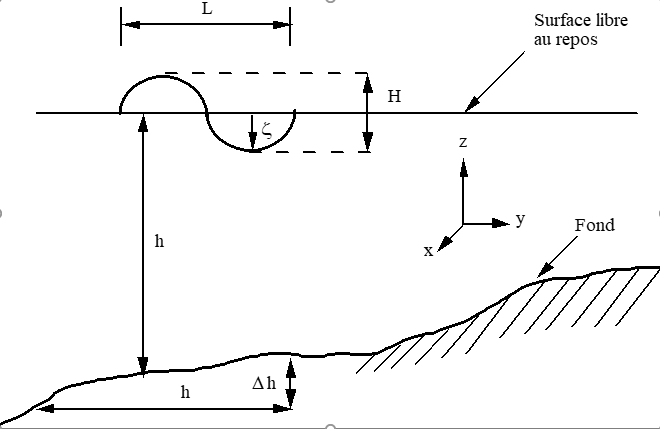
\includegraphics[scale=0.5,angle=0]{notations.png}
%   \caption{Notations: water depth $H(x,t)$, Free surface level $Z(x,t)$ and bottom level $Z_f(x,t)$.}
%   \label{fig:notations}
%  \end{center}
% \end{figure}

The system of equations (\ref{eq:NS_2d1}) to (\ref{eq:NS_2d3}) is supplemented by the following boundary conditions. If $n_s$ is the normal to the free surface and $n_b$ the normal to the bed surface :

\begin{equation}
 n_s = \frac{1}{\displaystyle  \sqrt{1 + \left( \frac{\partial z}{\partial x}\right)^2} }  \left( \begin{array}{c} -\frac{\partial z}{\partial x}\\ \\ 1 \end{array} \right)
\end{equation}

and

\begin{equation}
 n_b = \frac{1}{\displaystyle \sqrt{1 + \left( \frac{\partial z_b}{\partial x}\right)^2}}  \left(\begin{array}{c} -\frac{\partial z_b}{\partial x}\\ \\ 1 \end{array} \right)
\end{equation}

%...............................................................................
\subsubsection{At the free surface}
%...............................................................................

The boundary condition at the free surface is a traditional kinematic condition :
\begin{equation}
\frac{\partial Z}{\partial t} + u_s \frac{\partial Z}{\partial x}
-w_s = 0
\label{eq:free_surf}
\end{equation}
where subscript $s$ indicates the value of the variable at the free surface.

%...............................................................................
\subsubsection{At the bottom}
%...............................................................................

\begin{equation}
 u_f \frac{\partial z_b}{\partial x}-w_f = 0
 \label{eq:bottom}
\end{equation}

where subscript $b$ indicates that the value of the variable is taken at the bottom.

The notations here are the same as those introduced in the previous section about the transcritical engine of \mascaret{}.

\begin{eqnarray}
 S(x,t) & = & \int_{l_{1}}^{l_{2}}h(x,y,t)dy \\
 \bar{u}(x,t) & = & \frac{1}{S(x,t)}\int_{l_{1}}^{l_{2}}\int_{Z_{b}}^{Z(x,t)}u(x,y,z,t)dzdy \\
 Q(x,t) & = & S(x,t)\bar{u}(x,t)
\end{eqnarray}

Integration along the vertical of the continuity equation (\ref{eq:NS_2d1}), with the boundary conditions defined by (\ref{eq:free_surf}) and (\ref{eq:bottom}), gives :

\begin{equation}
  \frac{\partial{S}}{\partial{t}}+\frac{\partial{Q}}{\partial{x}}=0 \label{eq:STV_1d1}\\
\end{equation}

Integration of equation (\ref{eq:NS_2d3}) gives the expression of the pressure.

\begin{equation}
  p(x,z,t)=p^{a}+g(Z(x,t)-z(x,t))+\int_{z}^{Z}{\frac{\partial{w}}{\partial{t}}}dz
\end{equation}

With the assumption that the pressure is hydrostatic, the term which depends on the vertical velocity component is not taken into account. It is also noted that only the term corresponding to the temporal derivative of the vertical velocity component is considered. The advective terms are here neglected. Integration along the vertical of the momentum equation (\ref{eq:NS_2d2}) gives the following equation :

\begin{equation}
\frac{\partial{Q}}{\partial{t}}+\frac{\partial{Q^{2}}}{\partial{x}}+g\int_{l_{1}}^{l_{2}}h\frac{\partial{Z}}{\partial{x}}dy+D =0
\label{eq:mod_cont}
\end{equation}

The friction terms are neglected. $D$ represents part of the non-hydrostatic terms, which are developed in the following section.

%...............................................................................
\subsubsection{Development of the non-hydrostatic terms}
%...............................................................................

\begin{equation}
D=\int_{l_{1}}^{l_{2}}\int_{Z_{b}}^{Z(t)}{\frac{\partial}{\partial{x}}}\left(\int_{z}^{Z(t)}{\frac{\partial{w}}{\partial{t}}dz_{1}}\right)dz
\label{eq:tnh}
\end{equation}

The velocity is such that its divergence equals zero (\ref{eq:NS_2d1}). Combined with the impermeability conditions at the bottom, the following expressions are obtained :

\begin{eqnarray}
w(z) & = & - \frac{\partial}{\partial{x}}\int_{Z_{b}}^{z}udz_1\\
     & = & - \frac{\partial}{\partial{x}}((z-Z_{b})\bar{u})\\
     & = & -(z-Z_{b})\frac{\partial{\bar{u}}}{\partial{x}}+\frac{\partial{Z_b}}{\partial{x}}\bar{u}
\label{expw}
\end{eqnarray}

If the expression for the vertical velocity component is incorporated in the term $D$, representing part of the non-hydrostatic terms, and if the Leibnitz rule is applied to (\ref{eq:tnh}), the following relation is obtained :

\begin{equation}
  D =\int_{l_{1}}^{l_{2}}\int_{Z_{b}}^{Z(t)}\left(\int_{z}^{Z(t)}\frac{\partial^2{w}}{\partial{x}\partial{t}}dz+\left.\frac{\partial{Z(t)}}{\partial{x}}\frac{\partial{w}}{\partial{t}}\right|_s\right)dzdy
\end{equation}

This relation is further developed when replacing the vertical velocity component by its expression (\ref{expw}).

\begin{eqnarray}
  D & = & -\frac{1}{2}\int_{l_{1}}^{l_{2}}\int_{Z_{b}}^{Z(t)}\left[{h}^2-{(z-Z_f)}^2\right]dzdy\frac{\partial^3{\bar{u}}}{\partial{{x}^2}\partial{t}} \\
    & + & 2\int_{l_{1}}^{l_{2}}\int_{Z_{b}}^{Z(t)}(Z-z)\frac{\partial{Z_f}}{\partial{x}}dzdy\frac{\partial^2{\bar{u}}}{\partial{x}\partial{t}} \nonumber \\
    & + & \int_{l_{1}}^{l_{2}}\int_{Z_{b}}^{Z(t)}(Z-z)\frac{\partial^2{Z_f}}{\partial^2{x}}dzdy\frac{\partial{\bar{u}}}{\partial{t}}\nonumber \\ & + & \int_{l_{1}}^{l_{2}}\int_{Z_{b}}^{Z(t)}h\frac{\partial{Z}}{\partial{x}}dzdy\frac{\partial^2{\bar{u}}}{\partial{x}\partial{t}}\nonumber \\
& + & \int_{l_{1}}^{l_{2}}\int_{Z_{b}}^{Z(t)}\frac{\partial{Z}}{\partial{x}}\frac{\partial{Z_f}}{\partial{x}}dzdy\frac{\partial{\bar{u}}}{\partial{t}} \nonumber
\end{eqnarray}

Not all the above terms are taken into account in the transcritical engine of \mascaret{}. Only the dominant term that does not contain bottom gradient terms is kept:

\begin{equation}
-\frac{1}{2}\int_{l_{1}}^{l_{2}}\int_{Z_{b}}^{Z(t)}\left[{h}^2-{(z-z_f)}^2\right]dzdy\frac{\partial^3{\bar{u}}}{\partial{{x}^2}\partial{t}}
\end{equation}

The double integral is expressed as follows :
\begin{eqnarray}
&&=\int_{Z_{b}}^{Z(t)}\left(\int_{l_{1}(z)}^{l_{2}(z)}\left[h^2-(z-Z_f)^2dy\right]dy\right)dz\\
&&=h^2\int_{Z_{b}}^{Z(t)}L(z)dz-\int_{Z_{b}}^{Z(t)}\left((z-Z_f)^2\right)L(z)dz\\
&&=h^2S(x,t)-\int_{Z_{b}}^{Z(t)}\left((z-Z_f)^2\right)L(z)dz
\end{eqnarray}

In the case of a channel with rectangular cross-section, the previous term is equal to $\frac{2}{3}Lh^3$.

The following term is added to the momentum equation of the Saint-Venant system to model some of the hydrostatic terms :

\begin{equation}
  \left(h^2S(x,t)-\int_{Z_{b}}^{Z(t)}\left((z-Z_f)^2\right)L(z)dz\right)\frac{\partial^3{\bar{u}}}{\partial{{x}^2}\partial{t}}
\end{equation}

The system of the Saint-Venant equations in 1D, for a real geometry, and accounting for the principal hydrostatic terms, can be written as below, when the advective terms are neglected in the expression of the pressure derivative with respect to $z$ (this assumption is justified with an asymptotic development, see \cite{BRISTEAU11}).

\begin{eqnarray}
\frac{\partial{S}}{\partial{t}}+\frac{\partial{Q}}{\partial{x}} & = & 0 \\
\frac{\partial{Q}}{\partial{t}}+\frac{\partial{Q^{2}}}{\partial{x}}+g\int_{l_{1}}^{l_{2}}h\frac{\partial{Z}}{\partial{x}}dy+D(x,t,\frac{\partial}{\partial{t}},\frac{\partial}{\partial{x}}) & = & 0 \\
D(x,t,\frac{\partial}{\partial{t}},\frac{\partial}{\partial{x}}) & = & \nonumber \\
\left(h^2S(x,t)-\int_{Z_{b}}^{Z(t)}\left((z-Z_f)^2\right)L(z)dz\right)\frac{\partial^3{\bar{u}}}{\partial{{x}^2}\partial{t}} & & \nonumber \\
& = & \alpha(x,t)\frac{\partial^3{\bar{u}}}{\partial{{x}^2}\partial{t}}
\label{eq:1}
\end{eqnarray}


%...............................................................................
\subsubsection{Discretisation of the non-hydrostatic terms}
%...............................................................................

This section presents the discretisation of the Saint-Venant system with the addition of the term $D$ defined by equation (\ref{eq:1}).

It shows how the non-hydrostatic terms with third order temporal and spatial derivatives of the velocity can be integrated relatively easily, starting with a numerical scheme of the finite volume type, and using a scheme of the predictor-corrector type.

The prediction step corresponds to the traditional Saint-Venant equations and provides the wetted cross-section at time $t^{n+1}$. This is then used with the flow in the correction step, taking the non-hydrostatic term into account. The finite volume scheme developed in this section is used for the Saint-Venant part of the equations.

It is assumed that the computational domain is discretised with $I$ nodes $x_i$.

$C_i$ is the cell of length $\Delta x_i=x_{i+1/2}-x_{i-1/2}$ with $x_{i+1/2}=(x_i+x_{i+1})/2$.
$X_i$ represents the average value of $X$ in cell $i$.

For the temporal discretisation, $t^n = \sum_{k < n} \Delta t^k$ where the time step $\Delta t^k$ is specified later on with a CFL condition.
The conservative part of the equations is computed with the finite volume numerical scheme used for transcritical flows. This conservative part also includes the source terms (bottom gradient and friction).

For clarity, the general structure of an explicit finite volume scheme is reminded below :

\begin{equation}
 \tilde{X}^{n+1}_i + D_i^{n+1} - \left(X^n_i + D_i^n\right) + \frac{\Delta t^n}{\Delta x_i}\left(F^n_{i+1/2} - F^n_{i-1/2}\right) = \Delta t^n S_b(X^n_i) \label{eq:model_dis}
\end{equation}

where $\tilde{X}=(S,Q)$, the numerical flux $F^n_{i+1/2}$ represents the flux as computed by the Roe scheme for the Saint-Venant equations and $S_b$ represents the source terms including friction and bottom gradients.
The term $\left(\alpha(x,t)\frac{\partial^3{\bar{u}}}{\partial{{x}^2}\partial{t}}\right)$ is taken into account at the next step.

The spatial derivatives of the velocity are expressed using traditional finite differences at time $t^{n+1}$ (respectively $t^n$).

\begin{equation}
\left(\alpha(x,t)\frac{\partial^2{\bar{u}}}{\partial{{x}^2}}\right)^{n+1}_{i}
=\alpha(x_i,t^{n+1})\left(\frac{\displaystyle \left(\frac{\partial{u}}{\partial{x}}\right)_{i+\frac{1}{2}}-\left(\frac{\partial{u}}{\partial{x}}\right)_{i-\frac{1}{2}}}{\Delta{x_i}}\right)^{n+1}
\end{equation}

where $u_i=\frac{Q_i}{S_i}$. $\left(\frac{\partial{u}}{\partial{x}}\right)_{i\mp\frac{1}{2}}$ is still to be evaluated. With a finite difference discretisation this gives in $i+\frac{1}{2}$ :

\begin{equation}
\frac{\displaystyle \frac{Q_{i+1}}{S_{i+1}}-\frac{Q_i}{S_i}}{\displaystyle \frac{\Delta{x_i}+\Delta{x_{i+1}}}{2}}
\end{equation}

All the terms in $n+1$ and those in $n$ are grouped, this gives a tridiagonal matrix to be solved.
The unknown of the system is the vector $(Q,S)^T$, given by the prediction step.


%...............................................................................
\subsubsection{Boundary conditions}
%...............................................................................

In a non-hydrostatic situation, boundary conditions are required for terms such as :
$$\frac{\partial^2 \overline{u}}{\partial x^2}\quad\mbox{and}\quad\frac{\partial \overline{u}}{\partial x}$$

Since there are no natural conditions, it is assumed that :

$$\frac{\partial \overline{u}}{\partial \underline{n}} = 0$$

$\underline{n}$ is the outgoing normal vector at the upstream and downstream boundaries of the domain.

